\mode*

\lecture[mem]{mem}{mem}

\section{Memory Addressing}

\subsection{Memory Addresses}

\begin{frame}{Three Kinds Of Addresses}
  \begin{center}
    \mode<beamer>{ \includegraphics[width=\textwidth]{addr-trans} }
    \mode<article>{ \includegraphics[width=.7\textwidth]{addr-trans} }
  \end{center}
\end{frame}

\begin{frame}[plain]
  \begin{center}
    \mode<beamer>{ \includegraphics[width=\textwidth]{memTranslate} }
    \mode<article>{ \includegraphics[width=.7\textwidth]{memTranslate} }
  \end{center}
\end{frame}

\begin{frame}{All CPUs Share The Same Memory}
  \begin{block}{Memory Arbiter}
    \begin{itemize}
    \item[if:] the chip is free
    \item[then:] grants access to a CPU
    \item[if:] the chip is busy servicing a request by another processor
    \item[then:] delay it
    \end{itemize}    
  \end{block}
  Even uniprocessor systems use memory arbiters because of \emph{DMA}.
\end{frame}

\subsection{Segmentation in Hardware}

\begin{frame}{Real Mode Address Translation}
  \begin{itemize}
  \item Backward compatibility of the processors
  \item BIOS uses real mode addressing
  \item Use 2 16-bit registers to get a 20-bit address
  \end{itemize}

  \begin{block}{Logical address format}
    \begin{center}
      \texttt{<segment:offset>}
    \end{center}
  \end{block}

  \begin{block}{Real mode address translation}
    $$\mathtt{segment\ number\times{}2^4+offset}$$
    \begin{itemize}
    \item[e.g.] to translate <\texttt{FFFF:0001}> into linear address:
      $$\mathtt{FFFF \times{} 16 + 0001 = FFFF0 + 0001 = FFFF1}$$
    \end{itemize}
  \end{block}
\end{frame}

See also: \citetitle[Sec.~2.4, \emph{16-bit CPU}]{wangshuang03}

\begin{frame}{Protected Mode Address Translation}
  \begin{center}
    \mode<beamer>{ \includegraphics[width=.8\textwidth]{osc-8-53} }
    \mode<article>{ \includegraphics[width=.5\textwidth]{osc-8-53} }
  \end{center}
\end{frame}

\begin{frame}{Segment Selectors}
  \begin{block}{A logical address consists of two parts:}
    \begin{center}
      \begin{tabular}{ccc}
        segment selector&:&offset\\
        {\scriptsize 16 bits}&&{\scriptsize 32 bits}
      \end{tabular}
    \end{center}
  \end{block}
  \begin{description}
  \item[Segment selector] is an index into GDT/LDT
  \end{description}
  \begin{center}
    \mode<beamer>{ \includegraphics[width=.8\textwidth]{seg-selector} }
    \mode<article>{ \includegraphics[width=.4\textwidth]{seg-selector} }
  \end{center}
\end{frame}

\begin{frame}{Segmentation Registers}
  \begin{block}{Segment registers hold segment selectors}
    \begin{description}
    \item[cs] code segment register
      \begin{itemize}
      \item[CPL] 2-bit, specifies the Current Privilege Level of the CPU
        \begin{itemize}
        \item[00] - Kernel mode
        \item[11] - User mode
        \end{itemize}
      \end{itemize}
    \item[ss] stack segment register
    \item[ds] data segment register
    \item[es/fs/gs] general purpose registers, may refer to arbitrary data segments
    \end{description}
  \end{block}
\end{frame}

See also:
\begin{itemize}
\item \citetitle[Sec.~6.3, \emph{Segment-Level Protection}]{intel86}
\item \citetitle{duarte:cpu-ring}
\end{itemize}


\begin{center}
  \includegraphics[width=.6\textwidth]{segmentProtection}
\end{center}

\begin{frame}{Segment Descriptors}
    All the segments are organized in 2 tables:
    \begin{description}
    \item[GDT] \emph{Global Descriptor Table}
      \begin{itemize}
      \item shared by all processes
      \item GDTR stores address and size of the GDT
      \end{itemize}
    \item[LDT] \emph{Local Descriptor Table}
      \begin{itemize}
      \item one process each
      \item LDTR stores address and size of the LDT
      \end{itemize}
    \item[Segment descriptors] are entries in either GDT or LDT, 8-byte long
    \end{description}
      \begin{block}{Analogy}
        \begin{center}
          \begin{tabular}{rcl}
            Process&$\Longleftrightarrow$&Process Descriptor(PCB)\\
            File&$\Longleftrightarrow$&Inode\\
            Segment&$\Longleftrightarrow$&Segment Descriptor
          \end{tabular}
        \end{center}
      \end{block}
\end{frame}

See also:
\begin{itemize}
\item Memory Translation And Segmentation \citetitle{duarte:mem}
\item \url{http://www.osdever.net/bkerndev/Docs/gdt.htm}
\item \href{http://www.jamesmolloy.co.uk/tutorial\_html/4.-The\%20GDT\%20and\%20IDT.html}{Sec 4} of \emph{JamesM's kernel development
    tutorials}\footnote{\url{http://www.jamesmolloy.co.uk/tutorial_html/4.-The\%20GDT\%20and\%20IDT.html}},
  The GDT and IDT
\end{itemize}

\begin{frame}[plain]%{Segment Descriptors}
  \begin{block}{Example: A LDT entry for code segment}
    \begin{center}
      \mode<beamer>{ \includegraphics[width=\textwidth]{mos-figs-4-44} }
      \mode<article>{ \includegraphics[width=.6\textwidth]{mos-figs-4-44} }
    \end{center}
  \end{block}
  {\small
    \begin{multicols}{2}
      \begin{itemize}
      \item[Base:] Where the segment starts
      \item[Limit:] 20 bit, $\Rightarrow{}2^{20}$ in size
      \item[G:] Granularity flag
        \begin{itemize}
        \item[0] - segment size in bytes
        \item[1] - in 4096 bytes
        \end{itemize}
      \item[S:] System flag
        \begin{itemize}
        \item[0] - system segment, e.g. LDT
        \item[1] - normal code/data segment
        \end{itemize}\columnbreak
      \item[D/B:]
        \begin{itemize}
        \item[0] - 16-bit offset
        \item[1] - 32-bit offset
        \end{itemize}
      \item[Type:] segment type (cs/ds/tss)
        \begin{itemize}
        \item[TSS:] Task status, i.e. it's executing or not
        \end{itemize}
      \item[DPL:] Descriptor Privilege Level. 0/3
      \item[P:] Segment-Present flag
        \begin{itemize}
        \item[0] - not in memory
        \item[1] - in memory
        \end{itemize}
      \item[AVL:] ignored by Linux
      \end{itemize}
    \end{multicols}}
\end{frame}

See: \citetitle[Sec.~6.3, \emph{Segment-Level Protection}, p108]{intel86}

\begin{center}
  \includegraphics[width=.6\textwidth]{gdt-entry2}
\end{center}

\begin{frame}{Fast Access to Segment Descriptors}
  \begin{block}{a non-programmable cache register for each segment register}
    \begin{center}
      \mode<beamer>{ \includegraphics[width=.8\textwidth]{nonprogrammable} }
      \mode<article>{ \includegraphics[width=.4\textwidth]{nonprogrammable} }
    \end{center}
  \end{block}
\end{frame}

\begin{frame}{Translating a logical address}
  \mode<beamer>{ \includegraphics[width=.7\textwidth]{logical2linear}
    \begin{tikzpicture}[remember picture, overlay]
      \node [scale=.9,text opacity=1,color=blue,xshift=8.5em,yshift=0em] at (current
      page.center) {1. $Index\times{}8+\text{table base}$};
      \node [scale=.9,text
      opacity=1,color=blue,xshift=9em,yshift=-2em] at (current page.center)
      {2. $\text{Descriptor base}+offset$};
    \end{tikzpicture}}
  \mode<article>{
    \begin{minipage}{.4\textwidth}
      \begin{enumerate}
      \item $Index\times{}8+table\ base$
      \item $Descriptor\ base+offset$
      \end{enumerate}
    \end{minipage}\qquad
    \begin{minipage}{.3\linewidth}
      \includegraphics[width=\textwidth]{logical2linear}
    \end{minipage}}
\end{frame}

\subsection{Segmentation in Linux}

\begin{frame}{Linux prefers paging to segmentation}
  \begin{block}{Because}
  \begin{itemize}
  \item Segmentation and paging are somewhat redundant
  \item Memory management is simpler when all processes share the same set of linear addresses
  \item Maximum portability. RISC architectures in particular have limited support for segmentation
  \end{itemize}
  \end{block}
  \textcolor{blue}{The Linux 2.6 uses segmentation only when required by the 80x86 architecture.}
\end{frame}

\begin{frame}{The Linux GDT Layout}
  \textcolor{blue}{Each GDT includes 18 segment descriptors and 14 null, unused, or
    reserved entries}
  \begin{block}{\texttt{include/asm-i386/segment.h}}
    \begin{scriptsize}\mode<beamer>{
      \begin{multicols}{3}
        \begin{itemize}
        \item[0] null
        \item[1] reserved
        \item[2] reserved
        \item[3] reserved
        \item[4] unused
        \item[5] unused
        \item[6] TLS segment \#1
        \item[7] TLS segment \#2
        \item[8] TLS segment \#3
        \item[9] reserved
        \item[10] reserved
        \item[11] reserved
        \item[12] \textcolor{blue}{kernel code segment}
        \item[13] \textcolor{blue}{kernel data segment}
        \item[14] \textcolor{blue}{default user CS}
        \item[15] \textcolor{blue}{default user DS}
        \item[16] \textcolor{blue}{TSS}
        \item[17] \textcolor{blue}{LDT}
        \item[18] PNPBIOS support
        \item[19] PNPBIOS support
        \item[20] PNPBIOS support
        \item[21] PNPBIOS support
        \item[22] PNPBIOS support
        \item[23] APM BIOS support
        \item[24] APM BIOS support
        \item[25] APM BIOS support
        \item[26] ESPFIX small SS
        \item[27] per-cpu
        \item[28] stack\_canary-20
        \item[29] unused
        \item[30] unused
        \item[31] TSS for double fault handler
        \end{itemize}
      \end{multicols}}\mode<article>{
      \begin{multicols}{4}
        \begin{itemize}
        \item[0] null
        \item[1] reserved
        \item[2] reserved
        \item[3] reserved
        \item[4] unused
        \item[5] unused
        \item[6] TLS segment \#1
        \item[7] TLS segment \#2
        \item[8] TLS segment \#3
        \item[9] reserved
        \item[10] reserved
        \item[11] reserved
        \item[12] \textcolor{blue}{kernel code segment}
        \item[13] \textcolor{blue}{kernel data segment}
        \item[14] \textcolor{blue}{default user CS}
        \item[15] \textcolor{blue}{default user DS}
        \item[16] \textcolor{blue}{TSS}
        \item[17] \textcolor{blue}{LDT}
        \item[18] PNPBIOS support
        \item[19] PNPBIOS support
        \item[20] PNPBIOS support
        \item[21] PNPBIOS support
        \item[22] PNPBIOS support
        \item[23] APM BIOS support
        \item[24] APM BIOS support
        \item[25] APM BIOS support
        \item[26] ESPFIX small SS
        \item[27] per-cpu
        \item[28] stack\_canary-20
        \item[29] unused
        \item[30] unused
        \item[31] TSS for double fault handler
        \end{itemize}
      \end{multicols}}
    \end{scriptsize}
  \end{block}
\end{frame}

Although Linux doesn't use hardware context switches, it is nonetheless forced to set up a
TSS for each distinct CPU in the system \citetitle[Sec.~3.3.2, \emph{Task State
  Segment}]{bovet2005understanding}. This is done for two main reasons:
\begin{itemize}
\item When an 80x86 CPU switches from User Mode to Kernel Mode, it fetches the address of
  the Kernel Mode stack from the TSS (see the sections ``\emph{Hardware Handling of
    Interrupts and Exceptions}'' in Chapter 4 and ``\emph{Issuing a System Call via the
    sysenter Instruction}'' in Chapter 10) \citetitle[Sec.~5, \emph{Inner-level stack
    pointers}]{wiki:tss}.
\item When a User Mode process attempts to access an I/O port by means of an \texttt{in}
  or \texttt{out} instruction, the CPU may need to access an I/O Permission Bitmap stored
  in the TSS to verify whether the process is allowed to address the port. \citetitle[Sec.~4,
  \emph{I/O port permissions}]{wiki:tss}
\end{itemize}

See also:
\begin{itemize}
\item \citetitle{wiki:gdt}
\item \citetitle[Sec.~2.3.2, \emph{The Linux LDTs}]{bovet2005understanding}
\end{itemize}

\begin{frame}{The Four Main Linux Segments}
  \begin{block}{Every process in Linux has these 4 segments}
    \begin{center}
      \begin{scriptsize}
        \begin{tabular}{|l|l|l|l|l|l|l|l|l|}
          \hline
          \textbf{Segment}&\textbf{Base}&\textbf{G}&\textbf{Limit}&\textbf{S}&\textbf{Type}&\textbf{DPL}&\textbf{D/B}&\textbf{P}\\\hline
          user code&\texttt{0x00000000}&1&\texttt{0xfffff}&1&10&3&1&1\\\hline
          user data&\texttt{0x00000000}&1&\texttt{0xfffff}&1&2&3&1&1\\\hline
          kernel code&\texttt{0x00000000}&1&\texttt{0xfffff}&1&10&0&1&1\\\hline
          kernel data&\texttt{0x00000000}&1&\texttt{0xfffff}&1&2&0&1&1\\\hline
        \end{tabular}
      \end{scriptsize}
    \end{center}
  \end{block}
    \begin{block}{All linear addresses start at 0, end at 4G-1}
    \begin{itemize}
    \item All processes share the same set of linear addresses
    \item Logical addresses coincide with linear addresses
    \end{itemize}
  \end{block}
\end{frame}

\begin{frame}{Segment Selectors}
  \begin{block}{\texttt{include/asm-i386/segment.h}}
    \begin{center}
      \mode<beamer>{ \includegraphics[width=\textwidth]{segment} }
      \mode<article>{ \includegraphics[width=.6\textwidth]{segment} }
    \end{center}
  \end{block}
  \begin{block}{$Selector = Index \ll 3 + G + RPL$}
    \begin{center}{\ttfamily
      \begin{tabular}{lll}
        \_\_USER\_CS& $14 \ll 3 + 3 = 115$& 0000 0000 0111 0011\\
        \_\_USER\_DS& $15 \ll 3 + 3 = 123$& 0000 0000 0111 1011\\
        \_\_KERNEL\_CS&$12 \ll 3 + 0 = 96$& 0000 0000 0110 0000\\
        \_\_KERNEL\_DS&$13 \ll 3 + 0 = 104$&0000 0000 0110 1000
      \end{tabular}}
    \end{center}
  \end{block}
\end{frame}

Values in segment registers:

\verbatimfont{\dejavu}
\begin{verbatim}
│          Index          │G:RPL│
├─┬─┬─┬─┬─┬─┬─┬─┬─┬─┬─┬─┬─┼─┬─┬─┤
│0 0 0 0 0 0 0 0 0 1 1 1 0│0│1 1│ __USER_CS   (14 << 3 + 3)
├─┼─┼─┼─┼─┼─┼─┼─┼─┼─┼─┼─┼─┼─┼─┼─┤                          
│0 0 0 0 0 0 0 0 0 1 1 1 1│0│1 1│ __USER_DS   (15 << 3 + 3)
├─┼─┼─┼─┼─┼─┼─┼─┼─┼─┼─┼─┼─┼─┼─┼─┤                          
│0 0 0 0 0 0 0 0 0 1 1 0 0│0│0 0│ __KERNEL_CS (12 << 3 + 0)
├─┼─┼─┼─┼─┼─┼─┼─┼─┼─┼─┼─┼─┼─┼─┼─┤                          
│0 0 0 0 0 0 0 0 0 1 1 0 1│0│0 0│ __KERNEL_DS (13 << 3 + 0)
└─┴─┴─┴─┴─┴─┴─┴─┴─┴─┴─┴─┴─┴─┴─┴─┘
\end{verbatim}
  
The corresponding Segment Selectors are defined by the macros \texttt{\_\_USER\_CS},
\texttt{\_\_USER\_DS}, \texttt{\_\_KERNEL\_CS}, and \texttt{\_\_KERNEL\_DS}, respectively. To
address the kernel code segment, for instance, the kernel just loads the value yielded by
the \texttt{\_\_KERNEL\_CS} macro into the \texttt{cs} segmentation register \citetitle[Sec.~2.3,
\emph{Segmentation in Linux}]{bovet2005understanding}.

Notice that the linear addresses associated with such segments all start at \texttt{0} and
reach the addressing limit of $2^{32}-1$. This means that all processes, either in User
Mode or in Kernel Mode, may use the same logical addresses.

Another important consequence of having all segments start at \texttt{0x00000000} is that in
Linux, logical addresses coincide with linear addresses; that is, the value of the Offset
field of a logical address always coincides with the value of the corresponding linear
address.

As stated earlier, the Current Privilege Level of the CPU indicates whether the processor
is in User or Kernel Mode and is specified by the RPL field of the Segment Selector stored
in the \texttt{cs} register. \emph{Whenever the CPL is changed, some segmentation registers
  must be correspondingly updated.} For instance, when the CPL is equal to 3 (User Mode),
the \texttt{ds} register must contain the Segment Selector of the user data segment, but
when the CPL is equal to 0, the \texttt{ds} register must contain the Segment Selector of
the kernel data segment.

A similar situation occurs for the \texttt{ss} register. It must refer to a User Mode stack
inside the user data segment when the CPL is 3, and it must refer to a Kernel Mode stack
inside the kernel data segment when the CPL is 0. \emph{When switching from User Mode to
  Kernel Mode, Linux always makes sure that the \texttt{ss} register contains the Segment
  Selector of the kernel data segment}.

When saving a pointer to an instruction or to a data structure, the kernel does not need
to store the Segment Selector component of the logical address, because the \texttt{ss}
register contains the current Segment Selector. As an example, when the kernel invokes a
function, it executes a \texttt{call} assembly language instruction specifying just the
Offset component of its logical address; the Segment Selector is implicitly selected as
the one referred to by the \texttt{cs} register. Because there is just one segment of type
"executable in Kernel Mode," namely the code segment identified by \texttt{\_\_KERNEL\_CS},
it is sufficient to load \texttt{\_\_KERNEL\_CS} into \texttt{cs} whenever the CPU switches to
Kernel Mode. The same argument goes for pointers to kernel data structures (implicitly
using the \texttt{ds} register), as well as for pointers to user data structures (the kernel
explicitly uses the \texttt{es} register).

\begin{frame}
  \begin{block}{Example:}
    To address the kernel code segment, the kernel just loads the value yielded by the
    {\texttt{\_\_KERNEL\_CS}} macro into the {\texttt{cs}} segmentation register.
  \end{block}
  \begin{block}{Note that}
    \begin{enumerate}
    \item \texttt{base = 0}
    \item \texttt{limit = 0xfffff}
    \end{enumerate}
    This means that
    \begin{itemize}
    \item all processes, either in User Mode or in Kernel Mode, may use the same
      logical addresses
    \item logical addresses (Offset fields) coincide with linear addresses
    \end{itemize}
  \end{block}
\end{frame}
  
\begin{frame}{The Linux GDT}{8 byte segment descriptor}
  \begin{center}
    \mode<beamer>{ \includegraphics[width=\textwidth]{gdt-entry} }
    \mode<article>{ \includegraphics[width=.6\textwidth]{gdt-entry} }
  \end{center}
  % \begin{block}{In \emph{include/asm-x86\_64/desc.h}}
  %   \includegraphics[width=\textwidth]{desc}
  % \end{block}
  \begin{block}{\texttt{arch/i386/kernel/head.S}}
    \begin{center}
      \mode<beamer>{ \includegraphics[width=\textwidth]{head3} }
      \mode<article>{ \includegraphics[width=.7\textwidth]{head3} }
    \end{center}
  \end{block}
\end{frame}

\begin{multicols}{2}
  \begin{itemize}
  \item $\mathtt{0x60 = 12 \ll 3 + 0}$
  \item $\mathtt{0x68 = 13 \ll 3 + 0}$
  \item $\mathtt{0x73 = 14 \ll 3 + 3}$
  \item $\mathtt{0x7b = 15 \ll 3 + 3}$
  \end{itemize}
\end{multicols}

From the comments of Memory Translation And Segmentation \citetitle{duarte:mem}:
\begin{itemize}
\item[Q:] I went to where the \texttt{gdt\_page} is instantiated
  (Line \href{http://lxr.linux.no/linux+v2.6.25.6/arch/x86/kernel/cpu/common.c\#L24}{24},
    \texttt{common.c}, 2.6.25)

  It has the following code:

  \texttt{[GDT\_ENTRY\_DEFAULT\_USER\_CS] = { { { 0x0000ffff, 0x00cffa00 } } }}

  Do you know what that means?
\item[A:] This line is building the 8-byte segment descriptor for the user code
  segment. To really follow it, there are 3 things you must bear in mind:
  \begin{enumerate}
  \item The x86 is little endian, meaning that for multi-byte data types (say, 32-bit or
    64-bit integers), the significance of bytes grows with memory address. If you declare
    a 32-bit integer as \texttt{0xdeadbeef}, then it would be laid out in memory like this
    (in hex, assuming memory addresses are growing to the right):
\begin{verbatim}
ef be ad de
lower => higher
\end{verbatim}
  \item In array declarations, or in this case a struct declaration, earlier elements go
    into lower memory addresses.
  \item The convention for Intel diagrams is to draw things with HIGHER memory addresses
    on the LEFT and on TOP. This is a bit counter intuitive, but I followed it to be
    consistent with Intel docs.
  \end{enumerate}
  When you put this all together, the declaration above will translate into the following
  bytes in memory, using Intel's ‘reversed’ notation:
\begin{verbatim}
(higher)
00 cf fa 00
00 00 ff ff
(lower)
\end{verbatim}
  If you compare these values against the segment descriptor diagram above, you'll see
  that: the ‘base’ fields are all zero, so the segment starts at \texttt{0x00000000}, the
  limit is \texttt{0xfffff} so the limit covers 4GB, byte 47-40 is \texttt{11111010}, so the
  DPL is 3 for ring 3.

  If you look into the Intel docs, they describe the fields I left grayed out. Hope this
  helps!
\end{itemize}

\begin{frame}
  \begin{center}
    \mode<beamer>{ \includegraphics[width=\textwidth]{gdt} }
    \mode<article>{ \includegraphics[width=.5\textwidth]{gdt} }
  \end{center}
  \mode<beamer>{
  \begin{tikzpicture}[remember picture, overlay]    
    \node [scale=.9,text opacity=1,color=blue,xshift=-10.15em,yshift=-11.5em]
    at (current page.center) {\textbf{cpu\_gdt\_table:} store all GDTs};
    \node [scale=.9,text opacity=1,color=blue,xshift=-3em,yshift=-13em]
    at (current page.center) {\textbf{cpu\_gdt\_descr:} store the addresses and sizes of the GDTs};
  \end{tikzpicture}}
\mode<article>{
  \begin{description}
    \item[cpu\_gdt\_table:] is an array of all GDTs
    \item[cpu\_gdt\_descr:] store the addresses and sizes of the GDTs
  \end{description}
}
\end{frame}

\subsection{Paging in Hardware}

\begin{frame}{Paging in Hardware}{Starting with the 80386, all 80x86 processors support paging}
  \begin{block}{A page is}
    \begin{itemize}
    \item a set of linear addresses
    \item a block of data
    \end{itemize}
  \end{block}
  \begin{block}{A page frame is}
    \begin{itemize}
    \item a constituent of main memory
    \item a storage area
    \end{itemize}
  \end{block}
  \begin{block}{A page table}
    \begin{itemize}
    \item is a data structure
    \item maps linear to physical addresses
    \item stored in main memory
    \end{itemize}
  \end{block}
\end{frame}

\begin{frame}{Pentium Paging}{Linear Address $\Rightarrow$ Physical Address}
  \begin{minipage}{.4\textwidth}
    \mbox{Two page size in Pentium:}
    \begin{small}
      \begin{itemize}
      \item[4K:] \mbox{2-level paging}% (Fig.~\ref{fig:2levelpaging})}
      \item[4M:] \mbox{1-level paging}% (Fig.~\ref{fig:paging})}
      \end{itemize}
    \end{small}
    \begin{center}
      \mode<beamer>{ \includegraphics[width=1.15\textwidth]{2-level-paging} }
      \mode<article>{ \includegraphics[width=.9\textwidth]{2-level-paging} }
    \end{center}
  \end{minipage}\qquad
  \begin{minipage}{.5\textwidth}
    \begin{center}
      \mode<beamer>{ \includegraphics[width=1.2\textwidth]{osc-8-54} }
      \mode<article>{ \includegraphics[width=.8\textwidth]{osc-8-54} }
    \end{center}
  \end{minipage}
\end{frame}

\begin{itemize}
\item The CR3 register points to the top level page table for the current process.
\end{itemize}

\begin{frame}%{ --- Intel i386}
  \begin{block}{Same structure for Page Dirs and Page Tables}
    \begin{itemize}
    \item 4 bytes (32 bits) long
    \item Page size is usually 4k ($2^{12}$ bytes). OS dependent
      \begin{itemize}
      \item[\$] \texttt{getconf PAGESIZE}
      \end{itemize}
    \item Could have $2^{32-12}=2^{20}=1M$ pages
      \begin{itemize}
      \item[] Could addressing $1M\times{}4KB=4GB$ memory
      \end{itemize}
    \end{itemize}
  \end{block}
  \begin{block}{Intel i386 page table entry}
    \begin{center}
      \mode<beamer>{ \includegraphics[width=.8\textwidth]{i386pte} }
      \mode<article>{ \includegraphics[width=.5\textwidth]{i386pte} }
    \end{center}
  \end{block}
\end{frame}

\begin{frame}{Physical Address Extension (PAE)}{32-bit linear$\Rightarrow{}$36-bit physical}
  \begin{block}{Need a new paging mechanism}
    \begin{scriptsize}
      \begin{center}
        \begin{tabular}{r|llllll}
          &Linear&Physical&Max&Page&PTE&Paging\\
          &Address&Address&RAM&Size&Size&Level\\\hline
          No PAE&32 bits&32 bits&$2^{32}=4GB$&4K,4M&32 bits&1,2\\
          PAE&32 bits&36 bits&$2^{36}=64GB$&4K,2M&64 bits&2,3
        \end{tabular}
      \end{center}
    \end{scriptsize}
  \end{block}
  \vspace{1em}
  \begin{minipage}{.49\textwidth}
    \begin{itemize}
    \item[PDPT] Page Directory Pointer Table, is a new level of Page Table
      \begin{itemize}
      \item[] $\texttt{64-bit entry}\times{}4$
      \end{itemize}
    \end{itemize}
  \end{minipage}\hfill
  \begin{minipage}{.49\textwidth}
    \begin{center}
      \mode<beamer>{ \includegraphics[width=\textwidth]{pae} }
      \mode<article>{ \includegraphics[width=.6\textwidth]{pae} }
    \end{center}
  \end{minipage}
\end{frame}

\begin{frame}{PAE with 4K pages}
  \begin{center}
    \mode<beamer>{ 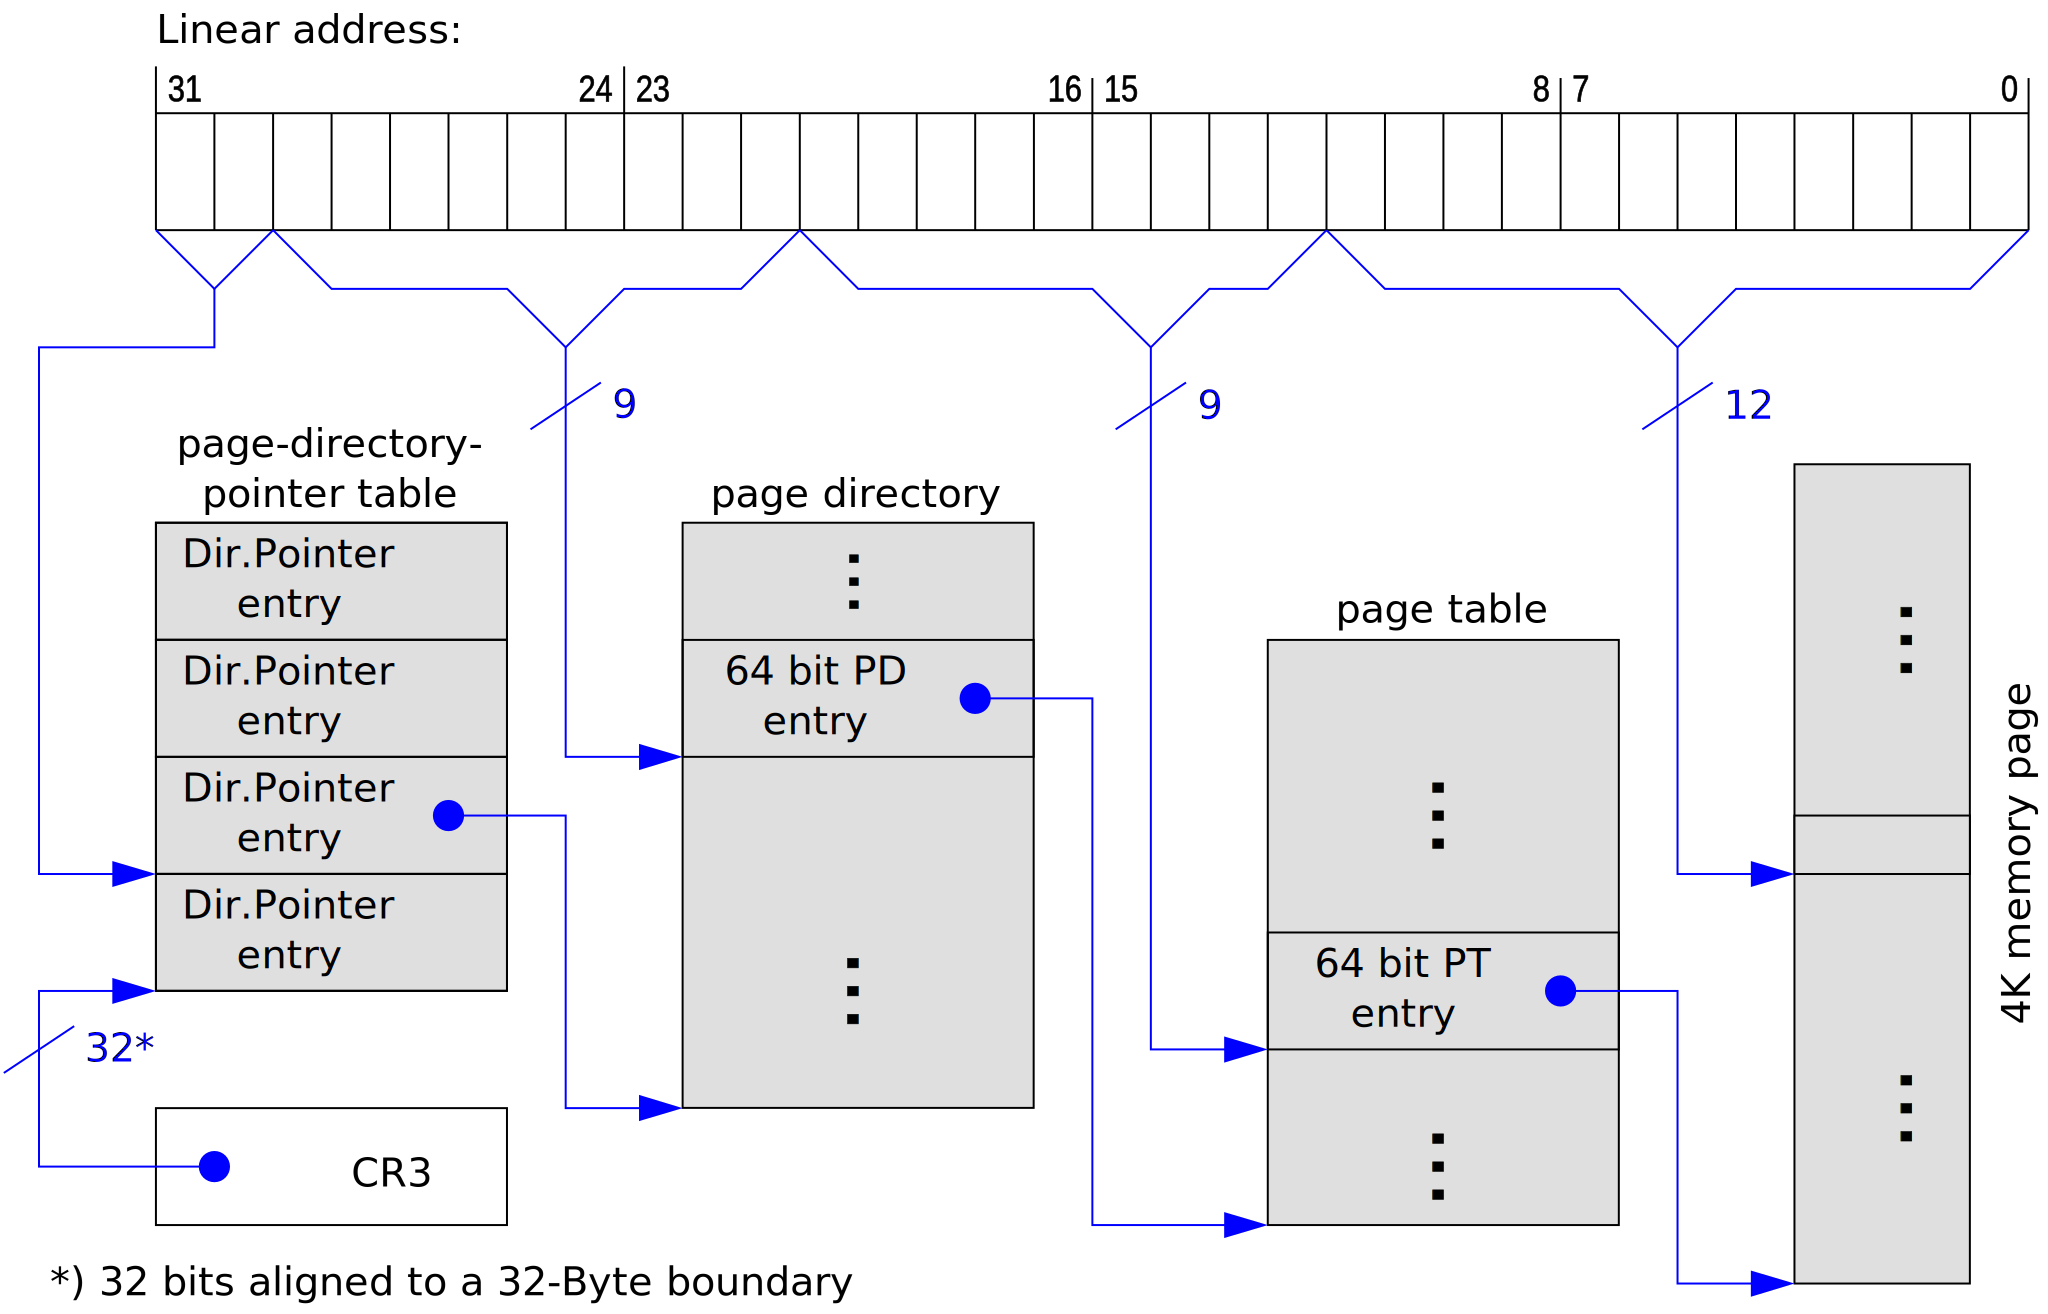
\includegraphics[width=\textwidth]{x86-pae-4k} }
    \mode<article>{ 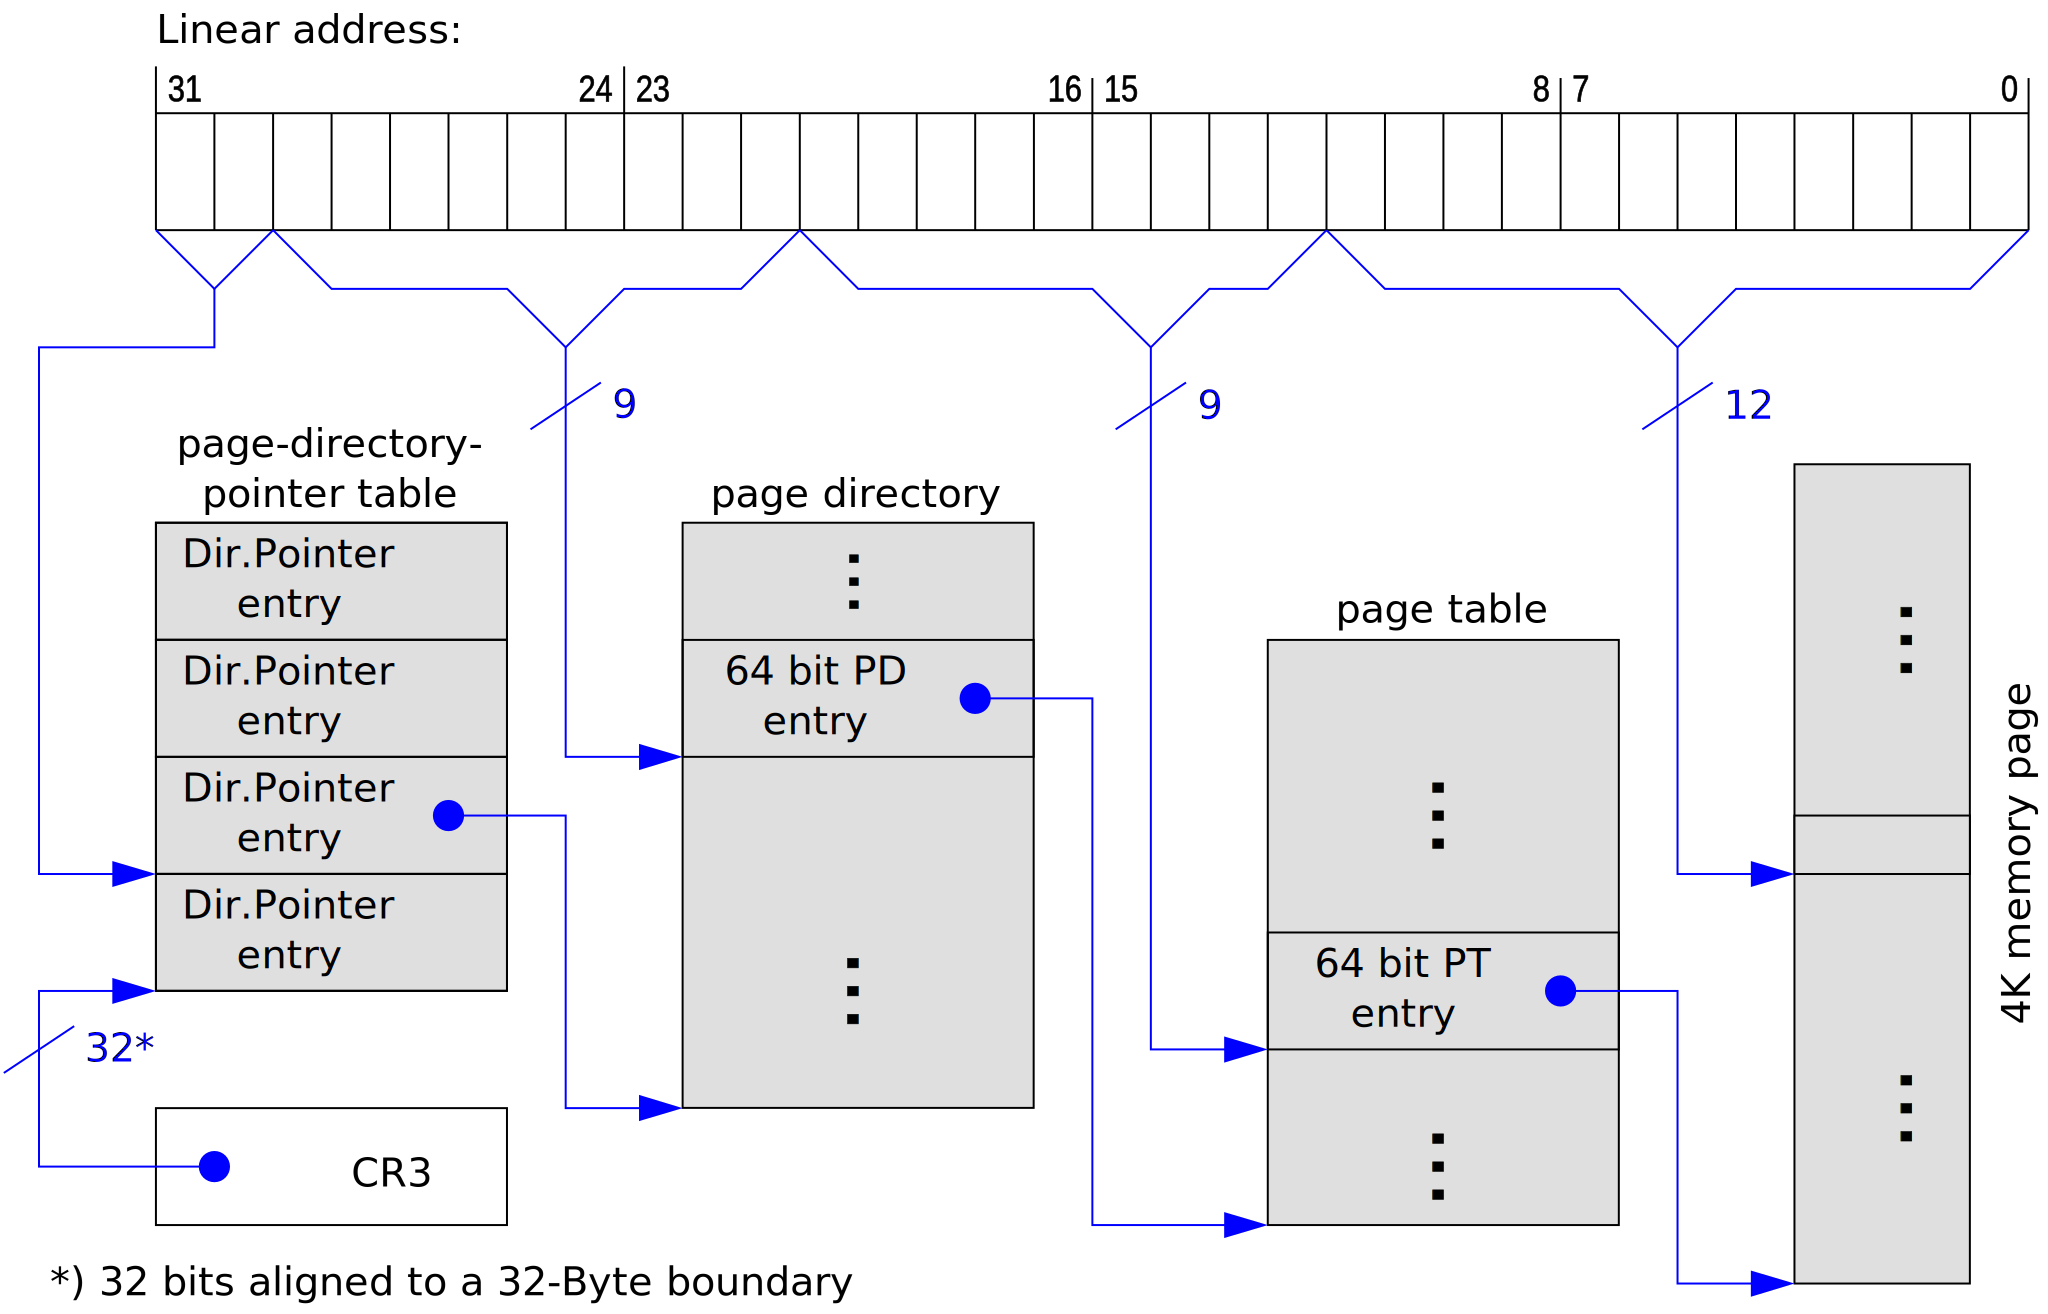
\includegraphics[width=.5\textwidth]{x86-pae-4k} }
  \end{center}
\end{frame}

\begin{frame}{PAE with 2M pages}
  \begin{center}
    \mode<beamer>{ \includegraphics[width=\textwidth]{x86-pae-2m} }
    \mode<article>{ \includegraphics[width=.5\textwidth]{x86-pae-2m} }
  \end{center}
\end{frame}

\begin{frame}{Physical Address Extension (PAE)}
  \begin{block}{The linear address are still 32 bits}
    \begin{itemize}
    \item A process cannot use more than 4G RAM
    \item The kernel programmers have to reuse the same linear addresses to map 64GB RAM
    \item The number of processes is increased
    \end{itemize}
  \end{block}
\end{frame}

\begin{frame}{Translation Lookaside Buffers (TLB)}
    \begin{block}{Fact: 80-20 rule}
    \begin{itemize}
    \item Only a small fraction of the PTEs are heavily read; the rest are barely used at
      all
    \end{itemize}
  \end{block}
  \begin{center}
    \mode<beamer>{ \includegraphics[width=.75\textwidth]{osc-8-28} }
    \mode<article>{ \includegraphics[width=.5\textwidth]{osc-8-28} }
  \end{center}
\end{frame}

\subsection{Paging in Linux}

\begin{frame}{Paging In Linux}{4-level paging for both 32-bit and 64-bit}
  \begin{center}
    \mode<beamer>{ \includegraphics[width=\textwidth]{4-level-paging} }
    \mode<article>{ \includegraphics[width=.5\textwidth]{4-level-paging} }
  \end{center}
  % \mode<beamer>{
  %   \begin{tikzpicture}[remember picture, overlay]    
  %     \node [scale=.7,xshift=-19.8em,yshift=-4em] (b) at (current page.center) {cr3};
  %     \draw [->,thick] (b) to[bend left] (.9,3.2);
  %   \end{tikzpicture}
  % }
  % \mode<article>{
  %   \textcolor{blue}{CR3} stores the starting address of PGDir for the current running
  %   process
  %   }
\end{frame}

\begin{frame}%{Paging In Linux}
  \begin{block}{4-level paging for both 32-bit and 64-bit}
    \begin{itemize}
    \item \textcolor{blue}{64-bit: four-level paging}
      \begin{multicols}{2}
        \begin{enumerate}
        \item Page Global Directory
        \item Page Upper Directory
        \item Page Middle Directory
        \item Page Table
        \end{enumerate}
      \end{multicols}
    \item \textcolor{blue}{32-bit: two-level paging}
      \begin{multicols}{2}
        \begin{enumerate}
        \item Page Global Directory
        \item Page Upper Directory --- 0 bits; 1 entry
        \item Page Middle Directory --- 0 bits; 1 entry
        \item Page Table
        \end{enumerate}
      \end{multicols}
    \end{itemize}
    \textcolor{blue}{The same code can work on 32-bit and 64-bit architectures}
  \end{block}
    \begin{center}
    \begin{scriptsize}
      \begin{tabular}{llllr}
        \hline
        &Page &Address&Paging&Address\\
        Arch&size &bits &levels&splitting\\\hline
        x86 &4KB(12bits) &32 &2 &$10+0+0+10+12$\\\hline
        x86-PAE&4KB(12bits)&32&3&$2+0+9+\hspace{.6em}9+12$\\\hline
        x86-64&4KB(12bits)&48&4&$9+9+9+\hspace{.6em}9+12$\\\hline    
      \end{tabular}
    \end{scriptsize}
  \end{center}
\end{frame}

For 32-bit architectures with no PAE, two paging levels are sufficient. Linux essentially
eliminates the PUD and the PMD fields by saying that they contain zero bits. However,
\emph{the positions of the PUD and the PMD in the sequence of pointers are kept so that
  the same code can work on 32-bit and 64-bit architectures}. \citetitle[Sec.~2.5,
\emph{Paging In Linux}]{bovet2005understanding}

\paragraph{Where are \emph{the sequence of pointers} kept?}

The kernel keeps a position for the PUD and the PMD by setting the number of entries in
them to 1 and mapping these two entries into the proper entry of the Page Global
Directory.

\paragraph{How can Linux use 4-level model, while Intel specifies 2-level paging? (32-bit
  no PAE)}

Quoted from \href{http://stackoverflow.com/questions/6627833/process-page-tables}{a stackoverflow page}\footnote{\url{http://stackoverflow.com/questions/6627833/process-page-tables}}:
\begin{quote}
  What I was trying to say was that the paging model used by the OS and the model used by
  the hardware are often distinct concepts. Linux uses a uniform paging model internally
  but this is layered on top of the hardware's paging model and requires architecture
  specific hacks to get it to work. It is the hardware's model that determines how address
  translation actually occurs (since it is the MMU that does this). \emph{Linux simply
    adds a layer of indirection on top. Deep in its bowels it still uses the 10:10:12
    model. --- Abhay Buch Jul 8 '11 at 22:58}
\end{quote}

\paragraph{More about paging}

Quoted from \url{http://linux-mm.org/VirtualMemory}:
\begin{quote}
  After bootup, all memory is accessed through the MMU which is paging enabled. So
  everything before and after \texttt{PAGE\_OFFSET} is paged. Not everything can be demand
  paged, though ... (since kernel data structures are resident). Pages below
  \texttt{PAGE\_OFFSET} belong to user space, and can be demand paged. Addresses above
  \texttt{PAGE\_OFFSET} are kernel memory. There is a linear mapping for the first 900 MB
  of kernel memory, where physical address 0 \char`~\, 896MB is mapped into
  \texttt{PAGE\_OFFSET} \char`~\, (\texttt{PAGE\_OFFSET} + 896MB). So there are 896M/4K
  physical frames addressable from \texttt{PAGE\_OFFSET} \char`~\, (\texttt{PAGE\_OFFSET} +
  896MB).

  Memory above \texttt{PAGE\_OFFSET} is kernel virtual memory. Part of it is a direct map of
  the first part of physical memory. \emph{but that same physical memory could also get
    virtual mappings from elsewhere}, eg. userspace or vmalloc. Also, userspace and
  vmalloc can map physical memory from outside the 896MB of direct mapped memory (as well
  as inside it).

  Most kernel memory allocation needs to come from that 896 MB, indeed, though page tables
  are the big exception ;) which means they're resident in memory all the time. Kernel
  data structures are always resident.

  Process page tables could be either inside the low 896MB, or in highmem (or some page
  tables in both - more likely).

  Physical memory is, by definition, not pageable. The contents of those pages might be
  pageable though. So you could have a page P at physical address 400MB. A process
  (eg. mozilla) is using that page at virtual address 120MB somewhere in its heap. The
  contents of the physical page can be paged out, at which point mozilla's heap page at
  120MB is paged out. But the kernel mapping (at \texttt{PAGE\_OFFSET} + 400MB) still maps
  the same page P just with different contents ;)
\end{quote}

\subsubsection{The Linear Address Fields}
    
\begin{frame}{The Linear Address Fields}
    \begin{center}
      \mode<beamer>{ \includegraphics[width=\textwidth]{shift} }
      \mode<article>{ \includegraphics[width=.5\textwidth]{shift} }
    \end{center}
  \begin{description}
  \item[\texttt{*\_SHIFT}] to specify the number of bits being mapped
  \item[\texttt{*\_MASK}] to mask out all the upper bits
  \item[\texttt{*\_SIZE}] how many bytes are addressed by each entry
  \end{description}
  \texttt{*\_MASK} and \texttt{*\_SIZE} values are calculated based on \texttt{*\_SHIFT}
\end{frame}

\begin{description}
\item[\texttt{PAGE\_SHIFT}:] Specifies the size of the area that a \emph{page table entry} can
  cover
\item[\texttt{PMD\_SHIFT}:] Specifies the size of the area that a \emph{PMD entry} can cover
  \begin{itemize}
  \item When PAE is disabled, \texttt{PMD\_SHIFT} yields the value 22 (12 from Offset plus 10 from
    Table)
  \item when PAE is enabled, \texttt{PMD\_SHIFT} yields the value 21 (12 from Offset plus 9 from
    Table)
  \item \texttt{LARGE\_PAGE\_SIZE = PMD\_SIZE}
    \begin{itemize}
    \item $2^{22}$, without PAE
    \item $2^{21}$, with PAE
    \end{itemize}
%    \includegraphics[width=4cm]{pae}
  \end{itemize}
\item[\texttt{PUD\_SHIFT}:] Specifies the size of the area that a \emph{PUD entry} can cover
  \begin{itemize}
  \item On the 80x86 processors, \texttt{PUD\_SHIFT} is always equal to \texttt{PMD\_SHIFT}
    \begin{itemize}
    \item because both PUD and PMD are 0-bit long
    \end{itemize}
  \item \texttt{PUD\_SIZE} is equal to 4MB or 2MB.
  \end{itemize}
\item[\texttt{PGDIR\_SHIFT}:] Specifies the size of the area that a \emph{PGDIR entry} can cover
  \begin{itemize}
  \item When PAE is disabled, \texttt{PGDIR\_SHIFT = PUD\_SHIFT = PMD\_SHIFT = 22}
  \item when PAE is enabled, \texttt{PGDIR\_SHIFT} $= 9_{PMD} + 9_{PT} + 12_{Offset} = 30$
  \end{itemize}
\end{description}

\begin{frame}%{Paging In Linux}{ --- The Linear Address Fields}
  \begin{block}{\texttt{include/asm-i386/page.h}}
    \begin{center}
      \mode<beamer>{ \includegraphics[width=\textwidth]{page} }
      \mode<article>{ \includegraphics[width=.5\textwidth]{page} }
    \end{center}
  \end{block}
  \begin{description}
  \item[\texttt{PAGE\_SIZE}:] $2^{12} = 4k$
  \item[\texttt{PAGE\_MASK}:] \texttt{0xfffff000}
  \item[\texttt{LARGE\_PAGE\_SIZE}:] depends
    \begin{itemize}
    \item[PAE:] $2^{21} = 2M$
    \item[no PAE:] $2^{22} = 4M$
    \end{itemize}
  \end{description}
\end{frame}

\begin{frame}{Compile Time Dual-mode}
  \begin{block}{\texttt{include/asm-i386/pgtable.h}}
    \begin{center}
      \mode<beamer>{ \includegraphics[width=\textwidth]{pgtable} }
      \mode<article>{ \includegraphics[width=.7\textwidth]{pgtable} }
    \end{center}
  \end{block}
  \begin{center}
    \begin{small}{\ttfamily
      \begin{tabular}{l|ccc}
        &PMD\_SHIFT&PUD\_SHIFT&PGDIR\_SHIFT\\\hline
        2-level&22&22&22\\
        3-level&21&21&30
      \end{tabular}}
    \end{small}
  \end{center}
  \begin{center}
    \mode<beamer>{ \includegraphics[width=\textwidth]{pgdir-shift} }
    \mode<article>{ \includegraphics[width=.7\textwidth]{pgdir-shift} }
  \end{center}
\end{frame}

\begin{frame}{2-level --- no PAE, 4K-page}
  \textcolor{blue}{PMD and PUD are folded}
  \begin{center}
    \mode<beamer>{ \includegraphics[width=.8\textwidth]{linear-addr-2level} }
    \mode<article>{ \includegraphics[width=.4\textwidth]{linear-addr-2level} }
  \end{center}
  \begin{block}{\texttt{include/asm-generic/pgtable-nopud.h}}
    \begin{center}
      \mode<beamer>{ \includegraphics[width=.7\textwidth]{pgtable-nopud} }
      \mode<article>{ \includegraphics[width=.4\textwidth]{pgtable-nopud} }
    \end{center}
  \end{block}
  \begin{block}{\texttt{include/asm-generic/pgtable-nopmd.h}}
    \begin{center}
      \mode<beamer>{ \includegraphics[width=.7\textwidth]{pgtable-nopmd} }
      \mode<article>{ \includegraphics[width=.4\textwidth]{pgtable-nopmd} }
    \end{center}
  \end{block}
\end{frame}

\begin{frame}[fragile=singleslide]{3-level --- PAE enabled}
  \begin{center}
    \mode<beamer>{ \includegraphics[width=.7\textwidth]{pae2} }
    \mode<article>{ \includegraphics[width=.3\textwidth]{pae2} }
  \end{center}
  \begin{block}{\texttt{include/asm-i386/pgtable-3level-defs.h}}
    \begin{center}
\begin{ccode}
#define PGDIR_SHIFT  30
#define PTRS_PER_PGD 4
#define PMD_SHIFT    21
#define PTRS_PER_PMD 512
\end{ccode}
    \end{center}
    % On the 80x86 processors, $\texttt{PUD\_SHIFT}= \texttt{PMD\_SHIFT}$
    \textcolor{blue}{PUD} is eliminated
  \end{block}
\end{frame}

\begin{frame}[fragile=singleslide]{4-level --- x86\_64}
  \begin{block}{48 address bits}
    \begin{center}
      \mode<beamer>{ \includegraphics[width=.9\textwidth]{linear-addr-64} }
      \mode<article>{ \includegraphics[width=.4\textwidth]{linear-addr-64} }
    \end{center}
  \end{block}
  \begin{block}{\texttt{include/asm-x86\_64/pgtable.h}}
    \begin{center}
\begin{ccode}
#define PGDIR_SHIFT  39
#define PTRS_PER_PGD 512

#define PUD_SHIFT    30
#define PTRS_PER_PUD 512

#define PMD_SHIFT    21
#define PTRS_PER_PMD 512
\end{ccode}
      % \mode<beamer>{
      %   \includegraphics[width=.7\textwidth]{pgtable-64}
      % }
      % \mode<article>{
      %   \includegraphics[width=.3\textwidth]{pgtable-64}
      % }
    \end{center}
  \end{block}
\end{frame}

\subsubsection{Page Table Handling}

\begin{frame}{Page Table Handling}{ --- Data formats}
  \begin{block}{\texttt{include/asm-i386/page.h}}
    \begin{center}
      \mode<beamer>{ \includegraphics[width=\textwidth]{page2} }
      \mode<article>{ \includegraphics[width=.8\textwidth]{page2} }
    \end{center}
  \end{block}
  % Two reasons to use \emph{struct}:
  % \begin{enumerate}
  % \item type protection
  % \item portability. It works with PAE which uses 4 more bits
  % \end{enumerate}
\end{frame}

\begin{description}
\item[Why structs?] \citetitle[p158]{mauerer2008professional} \texttt{structs} are used
  instead of elementary types to ensure that the contents of page table elements are
  handled only by the associated helper functions and never directly.
  
  \citetitle[Sec.~3.2, \emph{Describing a Page Table Entry}]{gorman2004understanding} Even
  though these are often just unsigned integers, they are defined as structs for two
  reasons. The first is for type protection so that they will not be used
  inappropriately. The second is for features like PAE...
\end{description}

\begin{itemize}
\item For 32-bit systems,
  \begin{itemize}
  \item long int: 4 bytes
  \item long long int: 8 bytes
  \end{itemize}
\item \texttt{pgprot\_t} holds the protection flags associated with a single entry.
  \begin{itemize}
  \item Present/RW/User/Accessed/Dirty...
  \end{itemize}
\item \texttt{\_\_pmd(x)}, type casting
\item \texttt{pmd\_val(x)}, reverse casting
\item \texttt{HPAGE\_SHIFT}, huge page shift.
  \begin{itemize}
  \item 22 - without PAE, page size is $2^{22}=4M$
  \item 21 - with PAE, page size is $2^{21}=2M$
  \end{itemize}
\end{itemize}

\begin{frame}{Page Table Handling}{Read or modify page table entries}
  \begin{block}{Macros and functions}
    \begin{scriptsize}
      \begin{center}{\ttfamily
        \begin{tabular}{llll}
          pte\_none&pte\_clear&set\_pte&pte\_same(a,b)\\
          pte\_present&pte\_user()&pte\_read()&pte\_write()\\
          pte\_exec()&pte\_dirty()&pte\_young()&pte\_file()\\
          mk\_pte\_huge()&pte\_wrprotect()&pte\_rdprotect()&pte\_exprotect()\\
          pte\_mkwrite()&pte\_mkread()&pte\_mkexec()&pte\_mkclean()\\
          pte\_mkdirty()&pte\_mkold()&pte\_mkyoung()&pte\_modify(p,v)\\
          mk\_pte(p,prot)&pte\_index(addr)&pte\_page(x)&pte\_to\_pgoff(pte)\\
        \end{tabular}}
      \end{center}
    \end{scriptsize}
  \end{block}
  \textcolor{blue}{a lot more for pmd, pud, pgd ...}
\end{frame}

\begin{frame}{Example --- To find a page table entry}{\texttt{mm/memory.c}}
  \begin{center}
    \mode<beamer>{ \includegraphics[width=.8\textwidth]{follow-page} }
    \mode<article>{ \includegraphics[width=.5\textwidth]{follow-page} }
  \end{center}
\end{frame}

\begin{description}
\item[\texttt{pgd\_offset(mm, addr)}] Receives as parameters the address of a memory
  descriptor \texttt{mm} \citetitle[Chapter 9, \emph{Process Address
    Space}]{bovet2005understanding} and a linear address \texttt{addr}. The macro yields
  the linear address of the entry in a Page Global Directory that corresponds to the
  address \texttt{addr}; the Page Global Directory is found through a pointer within the
  memory descriptor.
  \begin{description}
  \item[Memory descriptor] \citetitle[Sec 9.2, \emph{The Memory
      Descriptor}]{bovet2005understanding} All information related to the process address
    space is included in an object called the memory descriptor of type
    \texttt{mm\_struct}. This object is referenced by the \texttt{mm} field of the process
    descriptor.
  \end{description}

  Line \href{http://lxr.linux.no/linux+v2.6.11/include/asm-i386/pgtable.h\#L312}{312} in
  \texttt{pgtable.h}:
  \begin{center}
    \includegraphics[width=.7\textwidth]{pgd-offset}
  \end{center}

  Line \href{http://lxr.linux.no/linux+v2.6.11/include/asm-i386/pgtable.h\#L305}{305} in 
  \texttt{pgtable.h}:
  \begin{center}
    \includegraphics[width=.7\textwidth]{pgd-index}
  \end{center}

  \texttt{PTRS\_PER\_PGD} = $ \begin{cases}
    1024&\mathtt{i386, noPAE}\\
    4&\mathtt{i386, PAE}\\
    512&\mathtt{x86\_64}
  \end{cases}$

\item[\texttt{pud\_offset(pgd, addr)}] Receives as parameters a pointer \texttt{pgd} to a Page
  Global Directory entry and a linear address \texttt{addr}. The macro yields the linear
  address of the entry in a Page Upper Directory that corresponds to \texttt{addr}. In a
  two- or three-level paging system, this macro yields \texttt{pgd}, the address of a Page
  Global Directory entry.

  Line \href{http://lxr.linux.no/linux+v2.6.11/include/asm-generic/pgtable-nopud.h\#L36}{36} in
  \texttt{pgtable-nopud.h}:
  \begin{center}
    \includegraphics[width=.7\textwidth]{pud-offset}
  \end{center}

\item[\texttt{pmd\_offset(pud, addr)}] Receives as parameters a pointer \texttt{pud} to a Page
  Upper Directory entry and a linear address \texttt{addr}. The macro yields the address of the
  entry in a Page Middle Directory that corresponds to \texttt{addr}. In a two-level paging system,
  it yields \texttt{pud}, the address of a Page Global Directory entry.

  Line \href{http://lxr.linux.no/linux+v2.6.11/include/asm-generic/pgtable-nopmd.h\#L39}{39} in
  \texttt{pgtable-nopmd.h}:
  \begin{center}    
    \includegraphics[width=.7\textwidth]{pmd-offset}
  \end{center}


\item[\texttt{pte\_offset\_kernel(dir, addr)}] Yields the linear address of the Page Table
  that corresponds to the linear address \texttt{addr} mapped by the Page Middle Directory
  \texttt{dir}. Used only on the master kernel page tables (See also \citetitle[Sec.~2.5.5,
  \emph{Kernel Page Tables}]{bovet2005understanding}).

  Line \href{http://lxr.linux.no/linux+v2.6.11/include/asm-i386/pgtable.h\#L335}{335} in
  \texttt{pgtable.h}:
  \begin{center}
    \includegraphics[width=.7\textwidth]{pte-offset}
  \end{center}

\item[\texttt{pte\_offset\_map(dir, addr)}] Receives as parameters a pointer \texttt{dir} to a
  Page Middle Directory entry and a linear address \texttt{addr}; it yields the linear
  address of the entry in the Page Table that corresponds to the linear address
  \texttt{addr}. If the Page Table is kept in high memory, the kernel establishes a
  temporary kernel mapping (See also \citetitle[Sec.~8.1.6, \emph{Kernel Mappings
    of High-Memory Page Frames}]{bovet2005understanding}), to be released by means of
  \texttt{pte\_unmap}. The macros \texttt{pte\_offset\_map\_nested} and
  \texttt{pte\_unmap\_nested} are identical, but they use a different temporary kernel
  mapping.

  Line \href{http://lxr.linux.no/linux+v2.6.11/include/asm-i386/pgtable.h\#L370}{370} in
  \texttt{pgtable.h}:
  \begin{center}
    \includegraphics[width=.7\textwidth]{pte-offset-map}
  \end{center}

\item[\texttt{pte\_none, pmd\_none, pud\_none, pgd\_none}] yield the value 1 if the
  corresponding entry has the value 0; otherwise, they yield the value 0.
\item[\texttt{pmd\_bad, pud\_bad, pgd\_bad}] The \texttt{pmd\_bad} macro is used by functions to
  check Page Middle Directory entries passed as input parameters. It yields the value 1 if
  the entry points to a bad Page Table that is, if at least one of the following
  conditions applies:
  \begin{itemize}
  \item The page is not in main memory (Present flag cleared).
  \item The page allows only Read access (Read/Write flag cleared).
  \item Either Accessed or Dirty is cleared (Linux always forces these flags to be set for
    every existing Page Table).
  \end{itemize}
  The \texttt{pud\_bad} and \texttt{pgd\_bad} macros always yield 0. No \texttt{pte\_bad} macro is
  defined, because it is legal for a Page Table entry to refer to a page that is not
  present in main memory, not writable, or not accessible at all.
\end{description}

\subsubsection{Physical Memory Layout}

\begin{frame}{Physical Memory Layout}
  \begin{description}
  \item[\texttt{0x00100000}]--- The kernel starting point
  \end{description}
  \begin{minipage}{.49\textwidth}
    \begin{block}{Reserved page frames}
      \begin{itemize}
      \item unavailable to users
      \item kernel code and data structures
      \item no dynamic assignment, no swap out
      \end{itemize}
    \end{block}
    \textcolor{blue}{The kernel is loaded starting from the second megabyte (\texttt{0x00100000})
      in RAM}
    \begin{itemize}
    \item Page frame 0 --- BIOS
    \item $640K\sim{}1M$ --- the well-know hole
    \item \texttt{/proc/iomem}
    \end{itemize}
  \end{minipage}\hfill
  \begin{minipage}{.49\textwidth}
    \mode<beamer>{
      \includegraphics[width=\textwidth]{boot-mem}
    } \mode<article>{
      \includegraphics[width=.7\textwidth]{boot-mem}
    }
  \end{minipage}
\end{frame}

\paragraph{Why isn't the kernel loaded starting with the first available megabyte of RAM?}

\citetitle[Sec.~2.5.3, \emph{inline}]{bovet2005understanding} Well, the PC architecture has
several peculiarities that must be taken into account. For example:

\begin{itemize}
\item Page frame 0 is used by BIOS to store the system hardware configuration detected
  during the Power-On Self-Test(POST); the BIOS of many laptops, moreover, writes data on
  this page frame even after the system is initialized.
\item Physical addresses ranging from \texttt{0x000a0000} to \texttt{0x000fffff} are usually
  reserved to BIOS routines and to map the internal memory of ISA graphics cards. This
  area is the well-known hole from 640 KB to 1 MB in all IBM-compatible PCs: the physical
  addresses exist but they are reserved, and the corresponding page frames cannot be used
  by the operating system.
\item Additional page frames within the first megabyte may be reserved by specific
  computer models. For example, the IBM ThinkPad maps the \texttt{0xa0} page frame into
  the \texttt{0x9f} one.
\end{itemize}

\begin{frame}%{Physical Memory Layout}
  \begin{block}{While booting}
    \begin{enumerate}
    \item The kernel queries the BIOS for available physical address ranges
    \item \texttt{machine\_specific\_memory\_setup()} --- builds the physical addresses map
    \item \texttt{setup\_memory()} --- initializes a few variables that describe the
      kernel's physical memory layout
      \begin{itemize}
      \item \texttt{min\_low\_pfn, max\_low\_pfn, highstart\_pfn, highend\_pfn, max\_pfn}
      \end{itemize}
    \end{enumerate}
  \end{block}
\end{frame}

See also: \citetitle[Sec.~3.4, \emph{Memory Initialization Steps}]{mauerer2008professional}

\verbatimfont{\dejavu}
\begin{verbatim}
setup_arch
├─ machine_specific_memory_setup
├─ parse_early_param
├─ setup_memory
├─ paging_init
│  └─ pagetable_init
└─ zone_sizes_init
   ├─ add_active_range
   └─ free_area_init_nodes
\end{verbatim}

\begin{itemize}
\item \texttt{setup\_arch} is invoked from within \texttt{start\_kernel()}
\item \texttt{machine\_specific\_memory\_setup}: to create a list with the memory regions occupied by
the system and the free memory regions
\item \texttt{parse\_early\_param}: parsing commandline arguments like \texttt{mem=XXX[KkmM]}, \texttt{highmem=XXX[kKmM]}, or \texttt{memmap=XXX[KkmM]""@XXX[KkmM]} arguments
\item \texttt{setup\_memory}
  \begin{itemize}
  \item The number of physical pages available (per node) is determined.
  \item The bootmem allocator is initialized \citetitle[Sec.~3.4.3, \emph{Memory Management
      During The Boot Process}]{mauerer2008professional}
  \item Various memory areas are then reserved, for instance, for the initial RAM disk needed when
   running the first userspace processes.
  \end{itemize}
\item \texttt{paging\_init}: initializes the kernel page tables and enables paging
\item \texttt{pagetable\_init}: initializes the direct mapping of physical memory into the
  kernel address space. All page frames in low memory are directly mapped to the virtual
  memory region above \texttt{PAGE\_OFFSET}. \emph{This allows the kernel to address a
    good part of the available memory without having to deal with page tables anymore}.
\item \texttt{zone\_sizes\_init}: initializes the \texttt{pgdat\_t} instances of all nodes of
  the system
  \begin{enumerate}
  \item \texttt{add\_active\_range}: a comparatively simple list of the available physical
    memory is prepared
  \item \texttt{free\_area\_init\_nodes}: uses this information (got in above step) to
    prepare the full-blown kernel data structures
  \end{enumerate}
\end{itemize}

\begin{frame}{BIOS-Provided Physical Addresses Map}
  \begin{block}{Example --- a typical computer with 128MB RAM}
    \begin{small}
      \begin{center}{\ttfamily
        \begin{tabular}{lll}
          Start&End&Type\\\hline
          0x00000000       &0x0009ffff (640K)&Usable\\
          0x000f0000 (960K)&0x000fffff (1M-1)&Reserved\\
          0x00100000 (1M)  &0x07feffff&Usable\\
          0x07ff0000       &0x07ff2fff&ACPI data\\
          0x07ff3000       &0x07ffffff (128M)&ACPI NVS\\
          0xffff0000       &0xffffffff&Reserved
        \end{tabular}}
      \end{center}
    \end{small}
  \end{block}
\end{frame}

\begin{itemize}
\item The \emph{ACPI data} area stores information about the hardware devices of the system
  written by the BIOS in the POST phase; during the initialization phase, the kernel
  copies such information in a suitable kernel data structure, and then considers these
  page frames usable.
\item The \emph{ACPI NVS} area is mapped to ROM chips of the hardware devices, and hence
  cannot be used.
\item The physical address range starting from \texttt{0xffff0000} is marked as reserved,
  because it is mapped by the hardware to the BIOS's ROM chip \citetitle[\emph{Appendix
    A}]{bovet2005understanding}
\item Notice that the BIOS may not provide information for some physical address ranges
  (in the table, the range is \texttt{0x000a0000} to \texttt{0x000effff}). To be on the safe
  side, Linux assumes that such ranges are not usable.
\item The kernel might not see all physical memory reported by the BIOS: for instance, the
  kernel can address only 4GB of RAM if it has not been compiled with PAE support, even
  if a larger amount of physical memory is actually available.
\item \href{http://kerneldiy.com/blog/?p=209}{kernlediy.com: Boot Memory Allocator}
\item \citetitle[Sec.~3.4.3, \emph{Memory Management During The Boot
    Process}]{mauerer2008professional}
\end{itemize}

\begin{frame}
  \begin{block}{Variables describing the physical memory layout}
    \begin{scriptsize}
      \begin{center}{\ttfamily
        \begin{tabular}{lp{.7\textwidth}}\hline
          \textbf{Variable name}&\textbf{Description}\\\hline
          num\_physpages&Page frame number of the highest usable page frame\\\hline
          totalram\_pages&Total number of usable page frames\\\hline
          min\_low\_pfn&Page frame number of the first usable page frame after the kernel image in RAM\\\hline
          max\_pfn&Page frame number of the last usable page frame\\\hline
          max\_low\_pfn&Page frame number of the last page frame directly mapped by the kernel (low memory)\\\hline
          totalhigh\_pages&Total number of page frames not directly mapped by the kernel (high memory)\\\hline
          highstart\_pfn&Page frame number of the first page frame not directly mapped by the kernel\\\hline
          highend\_pfn&Page frame number of the last page frame not directly mapped by the kernel\\\hline
        \end{tabular}}
      \end{center}
    \end{scriptsize}
  \end{block}
\end{frame}

\begin{frame}%{Physical Memory Layout}
  \begin{block}{The first 768 page frames (3 MB) in Linux 2.6}
    \begin{center}
      \mode<beamer>{ \includegraphics[width=\textwidth]{mem-layout} }
      \mode<article>{ \includegraphics[width=.6\textwidth]{mem-layout} }
    \end{center}
  \end{block}
\end{frame}

\begin{itemize}
\item You can find the linear address of these symbols (\texttt{\_text, \_etext, \_edata,
    \_end}) in the file \texttt{System.map}, which is created right after the kernel is
  compiled.
\end{itemize}

\subsubsection{Process Page Tables}

\begin{frame}{Process Page Tables}
  \texttt{0xC0000000} $\Leftrightarrow$ \texttt{PAGE\_OFFSET}

  \begin{block}{\texttt{include/asm-i386/page.h}}
    \begin{center}
      \mode<beamer>{ \includegraphics[width=\textwidth]{page3} }
      \mode<article>{ \includegraphics[width=.7\textwidth]{page3} }
    \end{center}
  \end{block}
  \begin{center}
    \mode<beamer>{ \includegraphics[width=.6\textwidth]{process-linear-addr} }
    \mode<article>{ \includegraphics[width=.3\textwidth]{process-linear-addr} }
  \end{center}
  \begin{block}{Why?}
    \begin{itemize}
    \item easy to switch to kernel mode
    \item easy physical addressing due to direct mapping
      $$Physical = Virtual - \mathtt{PAGE\_OFFSET}$$
    \end{itemize}
  \end{block}
  % \begin{block}{include/asm-x86\_64/page.h}
  %   \includegraphics[width=\textwidth]{page4}
  % \end{block}
\end{frame}

\textbf{4G/4G solution}
\begin{itemize}
\item (\href{http://lwn.net/Articles/75174/}{LWN article}) There are users out there
  wanting to scale 32-bit Linux systems up to 32GB or more of main memory, so the
  enterprise-oriented Linux distributors have been scrambling to make that possible. One
  approach is the 4G/4G patch written by Ingo Molnar. This patch separates the kernel and
  user address spaces, allowing user processes to have 4GB of virtual memory while
  simultaneously expanding the kernel's low memory to 4GB. There is a cost, however:
  \emph{the translation buffer (TLB) is no longer shared and must be flushed for every
    transition between kernel and user space}. Estimates of the magnitude of the
  performance hit vary greatly, but numbers as high as 30\% have been thrown around. This
  option makes some systems work, however, so Red Hat ships a 4G/4G kernel with its
  enterprise offerings.

  Better solution: \textbf{go get a 64-bit system}.
\item (LWN article: \href{http://lwn.net/Articles/39283/}{4G/4G split on x86, 64 GB RAM
    (and more) support}) Performance impact of the 4G/4G feature:
  
  There's a runtime cost with the 4G/4G patch: to implement separate address spaces for
  the kernel and userspace VM, the entry/exit code has to switch between the kernel
  pagetables and the user pagetables. This causes TLB flushes, which are quite expensive,
  not so much in terms of TLB misses (which are quite fast on Intel CPUs if they come from
  caches), but in terms of the direct TLB flushing cost (\texttt{cr3} manipulation) done on
  system-entry. 
\item It would also be possible to get rid of the split completely by introducing two 4
  GiB address spaces, one for the kernel and one for each userspace program. However,
  context switches between kernel and user mode are more costly in this
  case. \citetitle[Sec~3.4.2,\emph{Initialization of Paging}, p175]{mauerer2008professional}
\end{itemize}

\textbf{Linux Memory Management Overview (a bit
  old)[\href{http://tldp.org/LDP/khg/HyperNews/get/memory/linuxmm.html}{tldp.org}]}
\begin{itemize}
\item A process' \texttt{PGDir} is initialized during a fork by
  \texttt{copy\_page\_tables()}. The idle process (\texttt{swapper}) has its \texttt{PGDir}
  initialized during the initialization sequence (\texttt{swapper\_pg\_dir}).
\item The kernel code and data segments are priveleged segments defined in the global
  descriptor table (GDT) and extend from 3 GB to 4 GB. The swapper page directory
  (\texttt{swapper\_pg\_dir}) is set up so that logical addresses and physical addresses are
  identical in kernel space.
\item Each user process has a local descriptor table (LDT) that contains a code segment and
  data-stack segment. These user segments extend from 0 to 3 GB (\texttt{0xc0000000}). In user
  space, linear addresses and logical addresses are identical.
\item The space above 3 GB appears in a process' \texttt{PGDir} as pointers (each entry in
  \texttt{PGDir} has a pointer) to kernel page tables. \citetitle[Sec 2.5.4, \emph{The entries of
    the PGDir}]{bovet2005understanding}

  This space is invisible to the process in user mode but the mapping becomes relevant
  when privileged mode is entered, for example, to handle a system call. Supervisor mode
  is entered within the context of the current process so address translation occurs with
  respect to the process' \texttt{PGDir} but using kernel segments. This is identically
  the mapping produced by using the \texttt{swapper\_pg\_dir} and kernel segments as both page
  directories use the same page tables in this space. Only \texttt{task[0]} (the idle task,
  sometimes called the swapper task for historical reasons, even though it has nothing to
  do with swapping in the Linux implementation) uses the \texttt{swapper\_pg\_dir} directly.
  \begin{itemize}
  \item The user process' \texttt{segment\_base = 0x00}, \texttt{page\_dir} private to the
    process.
  \item user process makes a system call: \texttt{segment\_base = 0xc0000000},
    \texttt{page\_dir = same user page\_dir}.
  \item \texttt{swapper\_pg\_dir} contains a mapping for all physical pages from
    \texttt{0xc0000000} to \texttt{0xc0000000 + end\_mem}, so the first 768 entries in
    \texttt{swapper\_pg\_dir} are 0's, and then there are 4 or more that point to kernel page
    tables.
  \item The user page directories have the same entries as \texttt{swapper\_pg\_dir} above
    768. The first 768 entries map the user space.
  \end{itemize}
\item The upshot is that whenever the linear address is above \texttt{0xc0000000} everything uses
  the same kernel page tables.
\item The user stack sits at the top of the user data segment and grows down. The kernel
  stack is not a pretty data structure or segment that I can point to with a ``yon lies
  the kernel stack.'' A \texttt{kernel\_stack\_frame} (a page) is associated with each newly
  created process and is used whenever the kernel operates within the context of that
  process. Bad things would happen if the kernel stack were to grow below its current
  stack frame.
\end{itemize}

\textbf{The entries of the PGDir} \citetitle[Sec.~2.5.4]{bovet2005understanding}

\begin{itemize}
\item lower than \texttt{0xc0000000}: (the first 768 entries with PAE disabled, or the first 3
  entries with PAE enabled) depends on the specific process
  \begin{itemize}
  \item Each user process thinks it has 3 GiB of memory
  \end{itemize}
\item higher than \texttt{0xc0000000}: can be addressed only when the process is in kernel
  mode. This address space is common to all the processes and equal to the corresponding
  entries of the master kernel PGDir (see the following section)
% \item The content of the first entries of the \code{PGDir} that map linear addresses lower
%   than \code{0xc0000000} (the first 768 entries with PAE disabled, or the first 3 entries
%   with PAE enabled) depends on the specific process. Conversely,
% \item the remaining entries should be the same for all processes and equal to the
%   corresponding entries of the master kernel Page Global Directory (see the following
%   section).
\item For 32-bit systems without PAE, \texttt{PGDir}
  \begin{itemize}
  \item is 10-bit long 
  \item has $2^{10}$ (1K) entries
  \item each PGDIR entry covers $2^{22}$ (4M)
  \item the first 768 entries cover $768\times{}2^{22}=3G$
  \end{itemize}
\item For 32-bit systems with PAE enabled, \texttt{PGDir}
  \begin{itemize}
  \item is 2-bit long
  \item has $2^2=4$ entries
  \item each \texttt{PGDIR} entry covers $2^{30} = 1G$
  \item the first 3 entries cover $3\times{}2^{30}=3G$
  \end{itemize}
\item The address space after \texttt{PAGE\_OFFSET} is reserved for the kernel and this is
  where the complete physical memory is mapped (eg. if a system has 64mb of RAM, it is
  mapped from \texttt{PAGE\_OFFSET} to \texttt{PAGE\_OFFSET + 64mb}). This address space is
  also used to map non-continuous physical memory into continuous virtual
  memory. \citetitle[Sec.~1.3.1, \emph{Significance of
    \texttt{PAGE\_OFFSET}}]{abhishek2002memory}
\end{itemize}

\subsubsection{Kernel Page Tables}

\begin{frame}{Kernel Page Tables}{Master Kernel Page Global Directory}
  \begin{center}
    \includegraphics[width=\textwidth]{kernel-page-table2}
  \end{center}
\end{frame}

\begin{frame}{In The Beginning, There Is No Paging}
  \begin{block}{Before tuning on paging, the page tables must be ready}
    Two phases:
    \begin{enumerate}
    \item \textbf{Bootstrapping:} sets up page tables for just 8MB so the paging unit can
      be enabled
      \begin{description}
      \item[8MB?] 2 page tables (pg0, pg1), enough to handle the kernel's code and data
        segments, and 128 KB for some dynamic data structures (page frame bitmap)
      \end{description}
    \item \textbf{Finalising:} initializes the rest of the page tables
    \end{enumerate}
  \end{block}  
\end{frame}

\begin{frame}[squeeze]{Provisional Page Global Directory}
  \begin{itemize}
  \item \textcolor{blue}{A provisional PGDir} is initialized statically during kernel
    compilation
    \begin{center}
      \mode<beamer>{ \includegraphics[width=.5\textwidth]{head2} }
      \mode<article>{ \includegraphics[width=.3\textwidth]{head2} }
    \end{center}
  \item \textcolor{blue}{The provisional PTs} are initialized by \texttt{startup\_32()} in
    \texttt{arch/i386/kernel/head.S}
  \item \texttt{swapper\_pg\_dir} --- A 4KB area for holding provisional PGDir
  \item provisional PGDir has only 4 useful entries: \texttt{0, 1, 0x300, 0x301}
  \end{itemize}
  \begin{block}{What's it for?}
    \begin{center}
      \begin{tabular}{r|c|l}
        Linear&&Physical\\\hline
        $0\sim{}8MB$&$\Rightarrow$&$0\sim{}8MB$\\
        $\mathtt{PAGE\_OFFSET}\sim(\mathtt{PAGE\_OFFSET}+8MB)$&\rotatebox{30}{$\Rightarrow$}&
      \end{tabular}
    \end{center}
    So that the kernel image ($<8MB$) in physical memory can be addressed in both real
    mode and protected mode.
  \end{block}
\end{frame}

\begin{itemize}
\item ``\mintinline{gas}{.fill 1024, 4, 0}'' initializes a 4K area for
  \texttt{swapper\_pg\_dir}\footnote{\texttt{.fill REPEAT, SIZE, VALUE}: This emits
    \texttt{REPEAT} copies of \texttt{SIZE} bytes.}.
\item \texttt{swapper\_pg\_dir} is at the beginning of BSS (uninitialized data area) because
  BSS is no longer used after system start up.
\item assuming that the kernel's segments, the provisional Page Tables, and the 128KB
  memory area fit in the first 8 MB of RAM.
\item In order to map 8 MB of RAM, two Page Tables are required.
\item \texttt{pg0} is right after the end of BSS (\texttt{\_end}).
\end{itemize}

We won't bother mentioning the Page Upper Directories and Page Middle Directories anymore,
because they are equated to Page Global Directory entries. PAE support is not enabled at
this stage.

The objective of this first phase of paging is \emph{to allow these 8 MB of
  physical RAM to be easily addressed both in real mode and protected mode}. Therefore,
the kernel must create a mapping from both the linear addresses \texttt{0x00000000} through
\texttt{0x007fffff} (8M) and the linear addresses \texttt{0xc0000000} through
\texttt{0xc07fffff} (8M) into the physical addresses \texttt{0x00000000} through
\texttt{0x007fffff}. In other words, the kernel during its first phase of initialization can
address the first 8 MB of RAM by either linear addresses identical to the physical ones or
8 MB worth of linear addresses, starting from \texttt{0xc0000000}.

\paragraph{Why?}
Quoted from \citetitle[Sec 1.3.2]{abhishek2002memory}

\begin{itemize}
  \item All pointers in the compiled kernel refer to addresses \texttt{> PAGE\_OFFSET}. That is,
    the kernel is linked under the assumption that its base address will be
    \texttt{start\_text} (I think; I don't have the code on hand at the moment), which is
    defined to be \texttt{PAGE\_OFFSET}+(some small constant, call it \texttt{C}).
  \item All the kernel bootstrap code (mostly real mode code) is linked assuming that its
    base address is \texttt{0+C}.
  \end{itemize}

  \texttt{head.S} is part of the bootstrap code. It's running in protected mode with paging
  turned off, so all addresses are physical. In particular, the instruction pointer is
  fetching instructions based on physical address. The instruction that turns on paging
  (\mintinline{gas}{movl %eax, %cr0}) is located, say, at some physical address \texttt{A}.

  As soon as we set the paging bit in \texttt{cr0}, paging is enabled, and starting at the
  very next instruction, all addressing, including instruction fetches, pass through the
  address translation mechanism (page tables), IOW, all addresses are henceforth
  virtual. That means that
  \begin{enumerate}
  \item We must have valid page tables, and
  \item Those tables must properly map the instruction pointer to the next instruction to
    be executed.
  \end{enumerate}
  That next instruction is physically located at address \texttt{A+4} (the address
  immediately after the
  "\mintinline{gas}{movl %eax, %cr0}" instruction), but from the point of
    view of all the kernel code --- which has been linked at \texttt{PAGE\_OFFSET} ---
    that instruction is located at virtual address \texttt{PAGE\_OFFSET+(A+4)}. Turning on
    paging, however, does not magically change the value of EIP (The value of EIP is still
    physically \texttt{A+4}, not \texttt{PAGE\_OFFSET+(A+4)} yet. But since paging is just
    enabled, CPU could pass \texttt{A+4} through address translation).  The CPU fetches
    the next instruction from \emph{virtual} address \texttt{A+4}; that instruction is the
    beginning of a short sequence that effectively relocates the instruction pointer to
    point to the code at \texttt{PAGE\_OFFSET+A+(something)}.

  But since the CPU is, for those few instructions, fetching instructions based on
  physical addresses but \emph{having those instructions pass through address translation},
  we must ensure that both the physical addresses and the virtual addresses are :
  \begin{enumerate}
  \item Valid virtual addresses, and
  \item Point to the same code.
  \end{enumerate}
  That means that at the very least, the initial page tables must
  \begin{enumerate}
  \item map virtual address \texttt{PAGE\_OFFSET+(A+4)} to physical address \texttt{(A+4)},
    and must
  \item map virtual address \texttt{A+4} to physical address \texttt{A+4}.
  \end{enumerate}
  This dual mapping for the first 8MB of physical RAM is exactly what the initial page
  tables accomplish. The 8MB initally mapped is more or less arbitrary. It's certain that
  no bootable kernel will be greater than 8MB in size. The identity mapping is discarded
  when the MM system gets initialized.

\begin{frame}{Provisional Page Table Initialization}
  \begin{block}{\texttt{arch/i386/kernel/head.S}}
    \begin{center}
      \mode<beamer>{ \includegraphics[width=\textwidth]{head5} }
      \mode<article>{ \includegraphics[width=.8\textwidth]{head5} }
    \end{center}
  \end{block}
\end{frame}

\begin{itemize}
\item The identity mapping is discarded when the MM system gets initialized.
\item \mintinline{c}{page_pde_offset = (__PAGE_OFFSET >> 20); /* 0xC00, the 3K point.*/}
  
  The \texttt{PGDir} is one page (4K) in size. It's divided into two parts:
  \begin{enumerate}
  \item first 3K (768 entries) for user mode
  \item last 1K (256 entries) for kernel mode
  \end{enumerate}
\item ``\mintinline{gas}{$(pg0 - __PAGE_OFFSET)}'' %$
  yields the physical address of \texttt{pg0} since here
  it is a linear address. Same case for %
  ``\mintinline{gas}{$(swapper_pg_dir - __PAGE_OFFSET)}'' %$
\item Registers:
  \begin{description}
  \item[\texttt{\%edi}] address of each page table entry, i.e. \texttt{pg0[0]..pg0[1023]},
    \texttt{pg1[0]..pg1[1023]}.
  \item[\texttt{\%edx}] address of \texttt{swapper\_pg\_dir[0]} and then to
    \texttt{swapper\_pg\_dir[1]}.
  \item[\texttt{\%ecx}] has two uses
    \begin{enumerate}
    \item contents of \texttt{swapper\_pg\_dir[0]}, \texttt{swapper\_pg\_dir[1]},
      \texttt{swapper\_pg\_dir[768]},\\ \texttt{swapper\_pg\_dir[769]}.
    \item loop counter (1024 -> 0)
    \end{enumerate}
  \item[\texttt{\%eax}] \texttt{7, 4k+7, 8k+7 ... 8M-4k+7} for 2k page table entries in
    \texttt{pg0} and \texttt{pg1} respectively.
  \item[\texttt{\%ebp}] \texttt{= 128k + 7 + \&pg0[1023]} in the first round of loop. Its
    value cannot be determined at coding time, because the address of \texttt{pg0} is
    not known until compile/link time.
  \end{description}
\item \texttt{stosl}: stores the contents of EAX at the address
  pointed by \texttt{EDI}, and increments \texttt{EDI}. Equivalent to:
  \begin{center}
\begin{gascode}
movl %eax, (%edi)
addl $4, %edi
\end{gascode}
  \end{center}
\item \texttt{cmpl, jb}: if \texttt{\%eax} < \texttt{\%ebp}, jump to 10;
  \begin{itemize}
  \item At the end of the 1\textsuperscript{st} round of loop, the value of \texttt{\%eax} is
    \texttt{4M-4k+7}, while the value of \texttt{\%ebp} depends on the address of \texttt{pg0}.
  \end{itemize}
\item \texttt{INIT\_MAP\_BEYOND\_END}: \texttt{128KB}\footnote{dead link: \url{http://kerneldiy.com/blog/?p=201}}
\end{itemize}

\begin{frame}
  \begin{block}{Equivalent pseudo C code}
    \begin{center}
      \mode<beamer>{ \includegraphics[width=\textwidth]{provisional-pgdir1} }
      \mode<article>{ \includegraphics[width=.7\textwidth]{provisional-pgdir1} }
    \end{center}
  \end{block}
\end{frame}

See also: \url{http://www.eefocus.com/article/09-04/71517s.html}

\begin{frame}{Enable paging}
  \texttt{startup\_32()} in \texttt{arch/i386/kernel/head.S}
  \begin{center}
    \mode<beamer>{ \includegraphics[width=\textwidth]{head6} }
    \mode<article>{ \includegraphics[width=.5\textwidth]{head6} }
  \end{center}
\end{frame}

\begin{frame}{Final Kernel Page Table Setup}
  \begin{itemize}
  \item \texttt{master kernel PGDir} is still in \texttt{swapper\_pg\_dir}
  \item initialized by \texttt{paging\_init()}
  \end{itemize}
  
  \begin{block}{Situations}
    \begin{enumerate}
    \item \textcolor{blue}{$\mathtt{RAM\ size} < 896M$}
      \begin{itemize}
      \item every RAM cell is mapped
      \end{itemize}
    \item \textcolor{blue}{$896M < \mathtt{RAM\ size} < 4G$}
      \begin{itemize}
      \item 896M are mapped
      \end{itemize}
    \item \textcolor{blue}{$\mathtt{RAM\ size} > 4G$}
      \begin{itemize}
      \item PAE enabled
      \end{itemize}
    \end{enumerate}
  \end{block}
\end{frame}

\begin{frame}{When RAM size is less than 896 MB}%{Final Kernel Page Table Setup}
  \begin{block}{\texttt{paging\_init()} without PAE}
    \begin{center}
      \mode<beamer>{ \includegraphics[width=.5\textwidth]{paging-init} }
      \mode<article>{ \includegraphics[width=.3\textwidth]{paging-init} }
    \end{center}
  \end{block}
\end{frame}

\begin{description}
\item[Is PAE enabled in your kernel?] try ``\mintinline{sh}{grep PAE /boot/config-*}''
\end{description}

\begin{itemize}
\item \noindent\texttt{paging\_init()} without PAE:
  \begin{enumerate}
  \item Invokes \texttt{pagetable\_init()} to set up the Page Table entries properly.
  \item Writes the physical address of \texttt{swapper\_pg\_dir} in the cr3 control register.
  \item Invokes \texttt{\_\_flush\_tlb\_all()} to invalidate all TLB entries.
  \end{enumerate}
\end{itemize}

\begin{frame}
  \begin{description}
  \item[2 level paging:] \texttt{PUD} and \texttt{PMD} are folded
  \end{description}
  \begin{center}
    \mode<beamer>{ \includegraphics[width=.7\textwidth]{linear-addr-2level} }
    \mode<article>{ \includegraphics[width=.4\textwidth]{linear-addr-2level} }
  \end{center}
  \begin{description}
  \item[\texttt{pagetable\_init()}] --- re-initializes the \texttt{PGDir} at
    \texttt{swapper\_pg\_dir}
  \item[Equivalent code:] 
  \end{description}
  \begin{center}
    \mode<beamer>{ \includegraphics[width=\textwidth]{pagetable-init1} }
    \mode<article>{ \includegraphics[width=.7\textwidth]{pagetable-init1} }
  \end{center}
\end{frame}

\begin{itemize}
\item \citetitle[Sec.~2.5.5.2, \emph{Final kernel Page Table when RAM size is less than 896
    MB}]{bovet2005understanding}
\item This loop begins setting up valid PMD entries to point to. In the PAE case, pages
  are allocated with \texttt{alloc\_bootmem\_low\_pages()} and the PGD is set
  appropriately. Without PAE, there is no middle directory, so it is just “folded” back
  onto the PGD to preserve the illustion of a 3-level pagetable. \citetitle[Appendix C,
  \emph{Page Table Management}, p224]{gorman2004understanding}
\item \mintinline{c}{#define pgd_index(address) (((address) >> PGDIR_SHIFT) & (PTRS_PER_PGD-1))}
  \begin{itemize}
  \item \mintinline{c}{(PAGE_OFFSET >> PGDIR_SHIFT) & (PTRS_PER_PGD-1)} $\Rightarrow{}$
  \item \mintinline{c}{(C0000000 >> 22) & (1024 - 1) = 0x300 & 1023 = 768}
  \end{itemize}
\item \texttt{pgd} is a pointer initialized to the \texttt{pgd\_t} corresponding to the
  beginning of the kernel portion of the linear address space. The lower 768 entries are
  left alone for user space.
\item \texttt{one\_md\_table\_init()} is described in the comments of the source code. And
  it's easy to trace the calls in it to get a clear idea.

  Line \href{http://lxr.linux.no/linux+v2.6.11/arch/i386/mm/init.c\#L55}{55} in
  \texttt{mm/init.c}:
  \begin{center}
    \includegraphics[width=.7\textwidth]{one-md-table-init}
  \end{center}
\item \mintinline{c}{#define set_pmd(pmdptr, pmdval) (*(pmdptr) = (pmdval))}
\end{itemize}

\begin{frame}{When RAM Size Is Between 896MB $\sim$ 4096MB}
  \begin{description}
  \item[Physical memory zones:]
  \end{description}
  \begin{center}
    \mode<beamer>{
      \includegraphics[width=.3\textwidth]{zones}
    } \mode<article>{
      \includegraphics[width=.2\textwidth]{zones}
    }
  \end{center}
  \begin{description}
  \item[Direct mapping for \texttt{ZONE\_NORMAL}:]
  \end{description}
  \begin{center}
    \mode<beamer>{
      \includegraphics[width=\textwidth]{pa-va}
    } \mode<article>{
      \includegraphics[width=.6\textwidth]{pa-va}
    }
  \end{center}
\end{frame}

\begin{itemize}
\item To initialize the Page Global Directory, the kernel uses the same code as in the
  previous case.
\item The \texttt{\_\_pa} macro is used to convert a linear address starting from
  \texttt{PAGE\_OFFSET} to the corresponding physical address, while the \texttt{\_\_va} macro
  does the reverse.
\item \texttt{ZONE\_DMA} - Contains page frames of memory below 16 MB
\item \texttt{ZONE\_NORMAL} - Contains page frames of memory at and above 16 MB and below
  896 MB
\item \texttt{ZONE\_HIGHMEM} - Contains page frames of memory at and above 896 MB
\end{itemize}

\begin{frame}{High Memory}
  \begin{center}
    \mode<beamer>{ \includegraphics[width=.9\textwidth]{highmem} }
    \mode<article>{ \includegraphics[width=.4\textwidth]{highmem} }
  \end{center}
\end{frame}

\begin{itemize}
\item Coping with HighMemory \citetitle{linuxmm:highmemory}
  \begin{itemize}
  \item Memory above the physical address of 896MB are temporarily mapped into kernel
    virtual memory whenever the kernel needs to access that memory.
  \item Data which the kernel frequently needs to access is allocated in the lower 896MB
    of memory (\texttt{ZONE\_NORMAL}) and can be immediately accessed by the kernel (see
    Temporary mapping).
  \item Data which the kernel only needs to access occasionally, including page cache,
    process memory and page tables, are preferentially allocated from
    \texttt{ZONE\_HIGHMEM}.
  \item The system can have additional physical memory zones to deal with devices that can
    only perform DMA to a limited amount of physical memory, \texttt{ZONE\_DMA} and
    \texttt{ZONE\_DMA32}.
  \item Allocations and pageout pressure on the various memory zones need to be balanced
    (see Memory Balancing).
  \end{itemize}
\item (From comments in \href{High Memory In The Linux
    Kernel}{http://kerneltrap.org/node/2450}) \textbf{The whole 1\textsuperscript{st} GB
    of physical RAM is reserved for kernel use?} In fact, it is. The kernel has to have
  control over the whole memory. It's the kernel's job to allocate/deallocate RAM to
  processes.

  What the kernel does is, maps the entire available memory in its own space, so that it
  can access any memory region. It then gives out free pages to processes which need them.

  The userspace processes cannot of its own allocate a page to itself. It has to request
  the kernel to give it some memory area. Once the kernel has mapped a physical page in
  the process's space, it can use that extra memory.
\item To access physical memory between the range of 1GiB and 4GiB, the kernel temporarily
  maps pages from high memory into \texttt{ZONE\_NORMAL} with
  \texttt{kmap()}. \citetitle[Sec.~2.5, \emph{High Memory}]{gorman2004understanding}

  \textbf{Why?} \citetitle[Sec 8.1.6, \emph{Kernel Mappings of High-Memory Page
    Frames}]{bovet2005understanding} Page frames above the 896 MB boundary are not
  generally mapped in the 4\textsuperscript{th} GiB of the kernel linear address spaces,
  so the kernel is unable to directly access them. This implies that each page allocator
  function that returns the linear address of the assigned page frame doesn't work for
  high-memory page frames, that is, for page frames in the \texttt{ZONE\_HIGHMEM} memory
  zone.

  For instance, suppose that the kernel invoked
  \texttt{\_\_get\_free\_pages(GFP\_HIGHMEM,0)} to allocate a page frame in high memory. If
  the allocator assigned a page frame in high memory, \texttt{\_\_get\_free\_pages()} cannot
  return its linear address because it doesn't exist (there is no mapping between physical
  frame and virtual page); thus, the function returns NULL. In turn, the kernel cannot use
  the page frame; even worse, the page frame cannot be released because the kernel has
  lost track of it.

  Linux designers had to find some way to allow the kernel to exploit all the available
  RAM, up to the 64 GB supported by PAE. The approach adopted is the following:
  \begin{itemize}
  \item The allocation of high-memory page frames is done only through the
    \texttt{alloc\_pages()} function and its \texttt{alloc\_page()} shortcut. These functions
    do not return the linear address of the first allocated page frame, because if the
    page frame belongs to the high memory, such linear address simply does not
    exist. Instead, \emph{the functions return the linear address of the page descriptor
      of the first allocated page frame} \citetitle[Sec~8.1.1, \emph{Page
      Descriptors}]{bovet2005understanding}. These linear addresses always exist, because
    all page descriptors are allocated in low memory once and forever during the kernel
    initialization.
  \item Page frames in high memory that do not have a linear address cannot be accessed by
    the kernel. Therefore, part of the last 128 MB of the kernel linear address space is
    dedicated to mapping high-memory page frames. Of course, this kind of mapping is
    temporary, otherwise only 128 MB of high memory would be accessible. Instead, by
    recycling linear addresses the whole high memory can be accessed, although at
    different times.
  \end{itemize}
\item More about high memory:
  \begin{itemize}
  \item \citetitle[Sec.~1.8, \emph{Page Table Setup}]{abhishek2002memory}
  \item
    \href{http://stackoverflow.com/questions/4528568/how-does-the-linux-kernel-manage-less-than-1gb-physical-memory}{Stackoverflow:
      How does the linux kernel manage less than 1GB physical memory?}
  \item \url{http://www.cs.usfca.edu/~cruse/cs635/lesson04.ppt}
  \item \url{http://ilinuxkernel.com/?p=1013}
  \end{itemize}
\end{itemize}

\begin{frame}{When RAM Size Is More Than 4096MB (PAE)}
  \begin{block}{A 3-level paging model is used}
    \begin{center}
      \mode<beamer>{ \includegraphics[width=.7\textwidth]{pae2} }
      \mode<article>{ \includegraphics[width=.3\textwidth]{pae2} }
    \end{center}
  \end{block}
  \begin{center}
    \begin{tabular}{|c|c|c|c|c|}
      \hline
      PGDir&PUD&PMD&PT&OFFSET\\\hline
      2&0&9&9&12\\\hline
    \end{tabular}
  \end{center}
\end{frame}

\begin{frame}
  \begin{block}{The PGDir is initialized by a cycle equivalent to the following:}
    \begin{center}
      \mode<beamer>{ \includegraphics[width=\textwidth]{pgdir-init-pae1} }
      \mode<article>{ \includegraphics[width=.9\textwidth]{pgdir-init-pae2} }
    \end{center}
  \end{block}
\end{frame}

\begin{itemize}
\item \citetitle[Sec.~2.5.5.4, \emph{Final kernel Page Table when RAM size is more than 4096
    MB}]{bovet2005understanding}
\item this code can be used for both PAE and no-PAE situation. That's why the \texttt{for}
  loop
  \begin{center}
\begin{ccode}
    for (; i<PTRS_PER_PGD; ++i, ++pgd)
\end{ccode}
  \end{center}
  
  is used when \texttt{i=3, PTRS\_PER\_PGD=4}.
\item \texttt{pgd\_index(address)} returns the index of a PGDir entry
  \begin{center}
\begin{ccode}
#define pgd_index(address) (((address) >> PGDIR_SHIFT) & (PTRS_PER_PGD-1))
\end{ccode}
  \end{center}
  
  \begin{itemize}
  \item[$\Rightarrow$] \texttt{(C0000000 >> 30) \& (4 - 1)} = 3
  \end{itemize}

  When PAE is enabled, there are 4 entries in \texttt{PGDir}. The first 3 entries are for
  user linear address space. The 4\textsuperscript{th} entry is for kernel space.
\item \mintinline{c}|#define set_pgd(pgdptr, pgdval) set_pud((pud_t *)(pgdptr), (pud_t) { pgdval })|

  puds are folded into pgds so this doesn't get actually called, but the define is needed
  for a generic inline function.
  \begin{center}
\begin{ccode}
set_pgd(swapper_pg_dir + i, __pgd(__pa(empty_zero_page) + 0x001));
\end{ccode}
  \end{center}
  
  The kernel initializes the first three entries in the \texttt{PGDir} corresponding to the
  user linear address space with the address of an empty page (\texttt{empty\_zero\_page}).

  Line \href{http://lxr.linux.no/linux+v2.6.11/arch/i386/kernel/head.S\#L417}{417} in
  \texttt{arch/i386/kernel/head.S}:
  \begin{center}
\begin{gascode}
ENTRY(empty_zero_page)
    .fill 4096,1,0
\end{gascode}
  \end{center}
\item The 4\textsuperscript{th} entry is initialized with the address of a \texttt{pmd}
  allocated by invoking \texttt{alloc\_bootmem\allowbreak\_low\_pages()}. There are 512
  entries in a \texttt{pmd},
  \begin{itemize}
  \item the first 448 entries are filled with the physical address of the first 896MB
    of RAM.
  \item the last 64 entries are reserved for noncontiguous memory allocation 
    \citetitle[Sec.~8.3, \emph{Noncontiguous Memory Area Management}]{bovet2005understanding}
  \end{itemize}
\end{itemize}

\subsubsection{Fix-Mapped Linear Addresses}

\begin{frame}{Division Of The Kernel Address Space}{On IA-32 Systems}
  \begin{center}
    \mode<beamer>{ \includegraphics[width=\textwidth]{kernel-addr-space} }
    \mode<article>{ \includegraphics[width=.7\textwidth]{kernel-addr-space} }
  \end{center}
  \begin{itemize}
  \item Virtually contiguous memory areas that are \emph{not} contiguous in physical
    memory can be reserved in the vmalloc area.
  \item \emph{Persistent mappings} are used for persistent kernel mapping of highmem page frames.
  \item \emph{Fixmaps} are virtual address space entries associated with a fixed but
    freely selectable page in physical address space.
  \end{itemize}
\end{frame}

\begin{description}
\item[\texttt{VMALLOC\_OFFSET}] 8MB. This gap acts as a safeguard against any kernel
  faults. If out of bound addresses are accessed (these are unintentional accesses to
  memory areas that are no longer physically present), access fails and an exception is
  generated to report the error. If the vmalloc area were to immediately follow the direct
  mappings, access would be successful and the error would not be noticed. There should be
  no need for this additional safeguard in stable operation, but it is useful when
  developing new kernel features that are not yet mature. \citetitle[Sec.~3.4.2,
  \emph{Architecture-Specific Setup}, p178]{mauerer2008professional}
\item[Fixmaps] The advantage of fixmap addresses is that at compilation
  time, the address acts like a constant whose physical address is assigned when the
  kernel is booted. Addresses of this kind can be de-referenced faster than when normal
  pointers are used. The kernel also ensures that the page table entries of fixmaps are
  not flushed from the TLB during a context switch so that access is always made via fast
  cache memory. \citetitle[Sec.~3.4.2, \emph{Architecture-Specific Setup},
  p180]{mauerer2008professional}
\end{description}

See also: \citetitle[Sec.~1.8.3, \emph{Fixmaps}]{abhishek2002memory}


% \subsubsection{Handling the Hardware Cache and the TLB}
% \label{sec:handl-hardw-cache}

\begin{center}
  \includegraphics[width=1.2\textwidth,angle=270]{big-pic}
\end{center}

\mode<all>
%%% Local Variables:
%%% mode: latex
%%% TeX-master: "kernel-b"
%%% End:
